% Created 2022-12-19 Mon 22:32
% Intended LaTeX compiler: pdflatex
\documentclass[openleft,oneside,showtrims]{memoir}
\usepackage{calc}

\setlength{\headwidth}{\textwidth}
\addtolength{\headwidth}{.382\foremargin}

\renewcommand\afterchapternum{}

\renewcommand\afterchaptertitle{%
\ifnum \c@secnumdepth>\m@ne%
\ifNoChapNum\else\par\nobreak\vskip\afterchapskip\fi%
\fi}

\setlength\beforechapskip{15pt}
\renewcommand\printchapternonum{\global\NoChapNumtrue}
\renewcommand{\chaptitlefont}{\raggedleft\normalfont\Huge\bfseries}
\makeatletter

\AtBeginDocument{
    \nonzeroparskip
    \frontmatter
}

\chapterstyle{lyhne}
\usepackage[utf8]{inputenc}
\usepackage[T1]{fontenc}
\usepackage{graphicx}
\usepackage{longtable}
\usepackage{wrapfig}
\usepackage{rotating}
\usepackage[normalem]{ulem}
\usepackage{amsmath}
\usepackage{amssymb}
\usepackage{capt-of}
\usepackage{hyperref}
\usepackage{listings}
\usepackage{parskip}
\usepackage{paralist}
\setcounter{secnumdepth}{3}
\author{Alisha Awen - Harmonic Alchemy Productions\thanks{Siren1@disroot.org}}
\date{\textit{<2022-10-19 Wed>}}
\title{HAP - Writing Resources}
\hypersetup{
 pdfauthor={Alisha Awen - Harmonic Alchemy Productions},
 pdftitle={HAP - Writing Resources},
 pdfkeywords={},
 pdfsubject={Harmonic Alchemy Productions - Modular Emacs - Writing Resources - A Guide for Independent Writers/Publishers. Everything you need to run an Independent Writing \& Publishing Operation, employing professional publishing industry standards, within a 100\% free as in Freedom, software infrastructure environment i.e., IPE (Integrated Publishing Environment). This implements common ``IDE'' concepts as applied to writing, planning, and publishing of written and/or performed literary works...  This guide also includes Templates and Instructions for using this ``Modular Emacs'' org-mode Document Editing and publishing system... Using the templates you are able to start up a book project that is turn key from start to finish! Turn key meaning a few typed keys to publish your book.. and other ``turn keys'' for writing, editing, planning, tracking...},
 pdfcreator={Emacs 28.2 (Org mode 9.5.5)}, 
 pdflang={English}}
\begin{document}

\maketitle
\setcounter{tocdepth}{3}
\tableofcontents

\chapter{📃 Preface: \emph{(or Introduction - Optional)}}
\label{sec:orgd221aa8}
\label{BOOK_PREFACE}
\texttt{Preface or Introduction Content:} 

Lorem Ipsum Lorem Ipsum dolor sit amet, consectetuer adipiscingelit. Duis tellus. Donec ante dolor, iaculis nec, gravidaac, cursus in, eros. Mauris vestibulum, felis et egestasullamcorper, purus nibh vehicula sem, eu egestas antenisl non justo. Fusce tincidunt, lorem nev dapibusconsectetuer, leo orci mollis ipsum, eget suscipit erospurus in ante.

At ipsum vitae est lacinia tincidunt. Maecenas elit orci,gravida ut, molestie non, venenatis vel, lorem. Sedlacinia. Suspendisse potenti. Sed ultricies cursuslectus. In id magna sit amet nibh suspicit euismod.Integer enim. Donec sapien ante, accumsan ut,sodales commodo, auctor quis, lacus. Maecenas a elitlacinia urna posuere sodales. Curabitur pede pede,molestie id, blandit vitae, varius ac, purus. Mauris atipsum vitae est lacinia tincidunt. Maecenas elit orci, gravida ut, molestie non, venenatis vel,lorem. Sed lacinia. Suspendisse potenti. Sed ultrucies cursus lectus. In id magna sit amet nibhsuspicit euismod. Integer enim. Donec sapien ante, accumsan ut, sodales commodo, auctorquis, lacus. Maecenas a elit lacinia urna posuere sodales. Curabitur pede pede, molestie id,blandit vitae, varius ac, purus.



\mainmatter
\chapter{Colour Symbolism}
\label{sec:org2362132}
\label{CHAPTER_colour-symbolism}
\section{Introduction:}
\label{sec:orge4dc9d5}

The following is an ever expanding list of colours and their symbolic meanings around the world... Starting out, only keywords are assigned in three categories:

\begin{itemize}
\item Neutral
\item Positive
\item Negative
\end{itemize}

Later, sections will be added to dive in deeper, (e.g., Variations based on segments of the general population, culture, race, spirituality, geographical location, etc.) All of these factors provide meaning into how people feel about colour, and how they are affected by it.

I may also create a story snippet section for each colour, treating the colour itself as if ``she'' were a character in a story.  This ``colourful character'' will visit different places, meet different people, and engage in some sort of plot or dialog, etc. All done in brief of course... 

The mini story will provide a ``first person'' experience of how people react to our ``colourful character'' based on the criteria in the first paragraph...

\section{Red:}
\label{sec:org1bb94dc}

\begin{figure}[htbp]
\centering

\includegraphics[width=300px]{./media/red-banner.png}
\caption{\label{fig:HAP-WR-001}RED (symbolic meanings)}
\end{figure}

\subsection{Neutral Attributes:}
\label{sec:orgfb9e379}

\begin{itemize}
\item Intense
\item Passionate
\item Hot
\item Fire
\item Blood
\end{itemize}

\subsection{Positive Attributes:}
\label{sec:org7936181}

\begin{itemize}
\item Excitement
\item Energy
\item Passion
\item Love
\item Sincerity
\item Happiness (Only in Japan)
\item Desire
\item Speed
\item Strength
\item Power
\end{itemize}

\subsection{Negative Attributes:}
\label{sec:org2fee72d}

\begin{itemize}
\item Aggression
\item Danger
\item Fire (distaster - destruction)
\item War
\item violence
\end{itemize}

\section{Pink:}
\label{sec:orgc10439a}

\begin{figure}[htbp]
\centering

\includegraphics[width=300px]{./media/pink-banner.png}
\caption{\label{fig:HAP-WR-002}PINK (symbolic meanings)}
\end{figure}

\subsection{Attributes: (all positive)}
\label{sec:org6d9e278}

\begin{itemize}
\item Love
\item Romance
\item Healing
\item Caring
\item Tenderness
\item Acceptance
\item Calm.
\end{itemize}

Pink is a unique colour... There are no negative attributes to this colour! It is also (for good reason) the colour visualized by Reiki Healing Practitioners. Hospital rooms should be painted with this colour... If a loved one is not feeling well, or angry with you, give them pink sweetheart roses to calm them, make them feel better, and/or accept your apology... Pink is truly a magic colour!

\section{Beige \& Ivory:}
\label{sec:org1701258}

\begin{figure}[htbp]
\centering

\includegraphics[width=300px]{./media/beige-ivory-banner.png}
\caption{\label{fig:HAP-WR-003}IVORY (symbolic meanings)}
\end{figure}

\subsection{Attributes: (all positive)}
\label{sec:orgdd7e03c}

\begin{itemize}
\item Unification
\item Quiet
\item Pleasantness
\item Calm
\item Simplicity
\end{itemize}

\section{Yellow:}
\label{sec:org8876b65}

\begin{figure}[htbp]
\centering

\includegraphics[width=300px]{./media/yellow-banner.png}
\caption{\label{fig:HAP-WR-004}YELLOW (symbolic meanings)}
\end{figure}

\subsection{Attributes:}
\label{sec:orgfdf0d50}

\subsubsection*{Neutral Attributes:}
\label{sec:orgecf06a8}

\begin{itemize}
\item Sunshine
\item Summer
\item Gold
\item Philosophy
\end{itemize}

\subsubsection*{Positive Attributes:}
\label{sec:org992845e}

\begin{itemize}
\item Joy
\item Happiness
\item Optimism
\item Idealism
\item Imagination
\item Hope
\item Friendship
\end{itemize}

\subsubsection*{Negative Attributes:}
\label{sec:org491f6da}

\begin{itemize}
\item Betrayal
\item Dishonesty
\item Cowardice
\item Jealousy
\item Covetousness
\item Deceit
\item Illness
\item Hazard
\end{itemize}

\section{Dark Blue:}
\label{sec:orge00220c}

\begin{figure}[htbp]
\centering

\includegraphics[width=300px]{./media/dark-blue-banner.png}
\caption{\label{fig:HAP-WR-005}DARK BLUE (symbolic meanings)}
\end{figure}

\subsection{Attributes:}
\label{sec:orgf76a231}

\subsubsection*{Neutral Attributes:}
\label{sec:org93b94ea}

\begin{itemize}
\item Integrity
\item Knowledge
\item Power
\item Seriousness
\end{itemize}

\section{Blue:}
\label{sec:orgd81aece}

\begin{figure}[htbp]
\centering

\includegraphics[width=300px]{./media/blue-banner.png}
\caption{\label{fig:HAP-WR-006}BLUE (symbolic meanings)}
\end{figure}

\subsection{Attributes:}
\label{sec:org689ed2f}

\subsubsection*{Neutral Attributes:}
\label{sec:org15b2bda}

\begin{itemize}
\item Sky
\item Water
\item Technology
\item Order
\item Truth
\item Cold
\item Calm
\end{itemize}

\subsubsection*{Positive Attributes:}
\label{sec:orgf7d6450}

\begin{itemize}
\item Peace
\item Tranquility
\item Stability
\item Security
\item Harmony
\item Loyalty
\item Unity
\item Trust
\item Confidence
\item Cleanliness
\end{itemize}

\subsubsection*{Negative Attributes:}
\label{sec:orgaf317d0}

\begin{itemize}
\item Conservatism
\item Depression
\item Appetite Suppressant
\end{itemize}

\section{Turquoise:}
\label{sec:org7285ef0}

\begin{figure}[htbp]
\centering

\includegraphics[width=300px]{./media/turquoise-banner.png}
\caption{\label{fig:HAP-WR-007}Turquoise (symbolic meanings)}
\end{figure}

\subsection{Attributes:}
\label{sec:orgb2d7907}

\subsubsection*{Neutral Attributes:}
\label{sec:org1b46a08}

\begin{itemize}
\item Calm
\end{itemize}

\subsubsection*{Variant Attributes:}
\label{sec:org007c868}

\begin{itemize}
\item Teal symbolizes sophistication
\item Aquamarine symbolizes water
\item Lighter turquoise has a feminine appeal
\end{itemize}

\section{Purple:}
\label{sec:orgff7b13d}

\begin{figure}[htbp]
\centering

\includegraphics[width=300px]{./media/purple-banner.png}
\caption{\label{fig:HAP-WR-008}Purple (symbolic meanings)}
\end{figure}

\subsection{Attributes:}
\label{sec:org2611a68}

\subsubsection*{Neutral Attributes:}
\label{sec:orgb8f6187}

\begin{itemize}
\item Royalty
\item Nobility
\item Ceremony
\item Mysterious
\item Transformation
\end{itemize}

\subsubsection*{Positive Attributes:}
\label{sec:org07b69f8}

\begin{itemize}
\item Honour
\item Temperance
\item Spirituality
\item Wisdom
\item Enlightenment
\end{itemize}

\subsubsection*{Negative Attributes:}
\label{sec:org81f699c}

\begin{itemize}
\item Cruelty
\item Arrogance
\item Mourning
\end{itemize}

\section{Lavender:}
\label{sec:org43b4d6c}

\begin{figure}[htbp]
\centering

\includegraphics[width=300px]{./media/lavender-banner.png}
\caption{\label{fig:HAP-WR-009}Lavender (symbolic meanings)}
\end{figure}

\subsection{Attributes:}
\label{sec:orgc0b2c64}

\subsubsection*{Neutral Attributes:}
\label{sec:org40a09f5}

\begin{itemize}
\item Femininity
\end{itemize}

\subsubsection*{Positive Attributes:}
\label{sec:org334f881}

\begin{itemize}
\item Grace
\item Elegance
\end{itemize}

\section{Orange:}
\label{sec:org39fb73e}

\begin{figure}[htbp]
\centering

\includegraphics[width=300px]{./media/orange-banner.png}
\caption{\label{fig:HAP-WR-010}Orange (symbolic meanings)}
\end{figure}

\subsection{Attributes:}
\label{sec:orga2c3aea}

\subsubsection*{Neutral Attributes:}
\label{sec:org6f9ede6}

\begin{itemize}
\item Energy
\item Vibrant
\item Expansive
\end{itemize}

\subsubsection*{Positive Attributes:}
\label{sec:orged1557e}

\begin{itemize}
\item Warmth
\item Balance
\item Enthusiasm
\end{itemize}

\subsubsection*{Negative Attributes:}
\label{sec:org3094cf4}

\begin{itemize}
\item Flamboyant
\item Demanding Attention
\end{itemize}

\section{Green:}
\label{sec:org2559226}

\begin{figure}[htbp]
\centering

\includegraphics[width=300px]{./media/green-banner.png}
\caption{\label{fig:HAP-WR-011}Green (symbolic meanings)}
\end{figure}

\subsection{Attributes:}
\label{sec:org7f1a85c}

\subsubsection*{Neutral Attributes:}
\label{sec:orgf49ce2c}

\begin{itemize}
\item Nature
\item Environment
\item Youth
\item Spring
\item Vigour
\end{itemize}

\subsubsection*{Positive Attributes:}
\label{sec:org9242831}

\begin{itemize}
\item Healthy
\item Good Luck
\item Renewal
\item Generosity
\item Fertility
\item Service
\end{itemize}

\subsubsection*{Negative Attributes:}
\label{sec:orgc596f70}

\begin{itemize}
\item Jealousy
\item Inexperience
\item Envy
\item Misfortune
\end{itemize}

\section{Brown:}
\label{sec:org4b3fe11}

\begin{figure}[htbp]
\centering

\includegraphics[width=300px]{./media/brown-banner.png}
\caption{\label{fig:HAP-WR-012}Brown (symbolic meanings)}
\end{figure}

\subsection{Attributes:}
\label{sec:org40dbfaa}

\subsubsection*{Neutral Attributes:}
\label{sec:orgd5c8f22}

\begin{itemize}
\item Earth
\item Outdoors
\item Endurance
\item Simplicity
\end{itemize}

\subsubsection*{Positive Attributes:}
\label{sec:orgda77f24}

\begin{itemize}
\item Stability
\item Hearth
\item Home
\item Reliability
\item Comfort
\end{itemize}

\subsubsection*{Negative Attributes:}
\label{sec:org139b201}

\begin{itemize}
\item Stuck
\item Burdensome
\item Immovable
\end{itemize}

\section{Gray:}
\label{sec:orgf2d5a24}

\begin{figure}[htbp]
\centering

\includegraphics[width=300px]{./media/gray-banner.png}
\caption{\label{fig:HAP-WR-013}Gray (symbolic meanings)}
\end{figure}

\subsection{Attributes:}
\label{sec:org3edc582}

\subsubsection*{Neutral Attributes:}
\label{sec:org3562e0a}

\begin{itemize}
\item Staid
\item Modesty
\item Solid
\item Conservative
\item Old Age
\end{itemize}

\subsubsection*{Positive Attributes:}
\label{sec:orgb468e01}

\begin{itemize}
\item Security
\item Reliability
\item Intelligence
\item Dignity
\item Maturity
\item Practical
\end{itemize}

\subsubsection*{Negative Attributes:}
\label{sec:org6418af6}

\begin{itemize}
\item Sadness
\item Boring
\end{itemize}

\subsubsection*{Variant Attributes:}
\label{sec:org20436e5}

\begin{itemize}
\item Silver symbolizes calm.
\end{itemize}

\section{White:}
\label{sec:orga422f16}

\begin{figure}[htbp]
\centering

\includegraphics[width=300px]{./media/white-banner.png}
\caption{\label{fig:HAP-WR-014}White (symbolic meanings)}
\end{figure}

\subsection{Attributes:}
\label{sec:org466e70e}

\subsubsection*{Neutral Attributes:}
\label{sec:org211866b}

\begin{itemize}
\item Cold
\item Clinical
\item Birth
\item Simplicity
\item Precision
\item Innocence
\item Youth
\item Winter
\item Snow
\end{itemize}

\subsubsection*{Positive Attributes:}
\label{sec:org6e5986a}

\begin{itemize}
\item Reverence
\item purity
\item Cleanliness
\item Peace
\item Humility
\item Good
\end{itemize}

\subsubsection*{Negative Attributes:}
\label{sec:org39e625d}

\begin{itemize}
\item Sterility
\end{itemize}

\subsubsection*{Cultural Attributes:}
\label{sec:org3f501e7}

\begin{itemize}
\item Marriage (Western cultures)
\item Death (Eastern cultures)
\end{itemize}

\section{Black:}
\label{sec:orgd331a6a}

\begin{figure}[htbp]
\centering

\includegraphics[width=300px]{./media/black-banner.png}
\caption{\label{fig:HAP-WR-015}Black (symbolic meanings)}
\end{figure}

\subsection{Attributes:}
\label{sec:org8fccc34}

\subsubsection*{Neutral Attributes:}
\label{sec:org5260fba}

\begin{itemize}
\item Austerity
\item Detachment
\item Formality
\item Mystery
\item Depth
\item Style
\item Anonymity
\item Underground
\end{itemize}

\subsubsection*{Positive Attributes:}
\label{sec:orga8304f1}

\begin{itemize}
\item Power
\item Sexuality
\item Sophistication
\item Elegance
\item Wealth
\end{itemize}

\subsubsection*{Negative Attributes:}
\label{sec:org8da6af8}

\begin{itemize}
\item Fear
\item Evil
\item Unhappiness
\item Mourning
\item Sadness
\item Remorse
\item Anger
\end{itemize}

\subsubsection*{Other Attributes:}
\label{sec:orgbc62103}

\begin{itemize}
\item Good technical color
\item Death (Western cultures)
\end{itemize}


\chapter{Short Story Structure}
\label{sec:org28b0f1a}
\label{CHAPTER_Short-Story-Structure}
\texttt{Article By: Philip Brewer} \emph{(reprinted here for convenience of Emacs Org-Mode users)... (see CREDITS above)}

There are a lot of models for story structure. They’re easy to apply to novels and feature-length films, but I found them hard to apply to short stories.

In fact, my early efforts to use formal models for story structure were so unsatisfactory, I seriously considered abandoning them as a tool for plotting short stories. I might have done so, except that the instructors teaching them were really smart people who knew I was working on short stories.

I believed that they were useful, but I wasn’t able to use them.
I attended Clarion this year. One thing I learned was a useful way to relate the formal models for story structure to the structure of a short story.

\section{Complete story structures}
\label{sec:org7ad4bc3}

The models I’m talking about are sometimes described as the structure of a “complete” story. In a real sense, this sort of structure is what makes a story a story, and not just an incident or a series of related scenes.  In fact, the case can be made human brains are hardwired to appreciate stories that are structured as complete stories.  Whether that’s true or not, since most stories are structured like this, people learn to view them as stories.

One good model for story structure (taught to me by Bruce Holland Rogers) is Algis Budrys’s seven point story structure. It has:

\begin{enumerate}
\item A character,

\item In a situation,

\item With a problem,

\item Who tries repeatedly to solve his problem,

\item But repeatedly fails, (usually making the problem worse),

\item Then, at the climax of the story, makes a final attempt (which might either succeed or fail, depending on the kind of story it is), after which

\item The result is “validated” in a way that makes it clear that what we saw was, in fact, the final result.
\end{enumerate}

Another good one (taught to me by Steven Barnes) is Joseph Campbell’s Hero’s Journey:

\begin{enumerate}
\item The hero is confronted with a challenge,

\item Rejects it,

\item But then is forced (or allowed) to accept it.

\item He travels on the road of trials,

\item Gathering powers and allies, and

\item Confronts evil—only to be defeated.

\item This leads to a dark night of the soul, after which

\item The hero makes a leap of faith that allows him to

\item Confront evil again and be victorious.

\item Finally, the student becomes the teacher.
\end{enumerate}

For a novel or a movie, it can work great to tell a full-blown complete story, with multiple unsuccessful attempts to solve the problem or many steps along the road of trials. But in a short story it’s really hard to get everything in.

After I first learned these story structures, I wrote several stories making a conscious effort to get the whole Hero’s Journey (or whole try-fail, try-fail, try-fail structure) in. I managed it (usually in six to eight thousand words), but the stories were fair at best. (While I was at Clarion, a couple of people workshopped stories with the whole Hero’s Journey in just a couple thousand words. It’s possible, but there’s not much room for anything else.)

I started looking at published stories in magazines, focusing on the stories that I really liked. Virtually none of them cranked through a whole Hero’s Journey or a whole “try-fail” story structure. Especially when I looked at award-winning stories, I just didn’t see many stories that followed those structures.

When I went to Clarion this year, I had two questions at the top of my list of things I wanted to learn:

\begin{enumerate}
\item What is the structure of a successful short story?

\item What is the relationship between that sort of story structure and “complete” story structures like the Hero’s Journey?
\end{enumerate}

I learned those two things out of order, so I’m going to talk about them out of order here. That actually works out well, because the answer to the second question implies the answer to the first question in a useful way.

\section{Short Stories}
\label{sec:orgd6c044a}

Steven Barnes showed us in class that pretty much every plotted story can be analyzed according to the Hero’s Journey. But, he explained, short stories tend to have parts of the structure pared down: Not all steps are shown in full-blown scenes.

It is important that the steps “take place” in the context of the story—that’s what makes it a story.  But it isn't necessary to show each step.  It is enough simply to mention them.  In fact, it can be enough simply to imply them.

Once I understood that, it became possible to match the structure of short stories to the 
models for story structure.

For example, lots of stories can be thought of as the first few steps on the Hero’s Journey: a challenge, a rejection of the challenge, and then an acceptance of the challenge. The acceptance of the challenge is the climax of the story. The “validation” segment of the story should imply the rest of the Hero’s Journey. The reader should end the story knowing that there will be a road of trials, that evil will be confronted, and so on.

Lots of other stories can be thought of as just the dark night of the soul and the leap of faith. The early steps along the hero’s journey can be filled in with flashbacks or simply implied by the circumstances of the characters as the story begins. However it happens, the reader needs to learn that the hero accepted the challenge, confronted evil, and was defeated. The story ends with the reader knowing that the hero will face evil again and this time be victorious.

I’m not quite sure why this was such a revelation to me. But, once I learned to see things this way, it suddenly became much easier to plot my own stories. It also became easier to explain plotting issues when critiquing other people’s stories.

It was less important to me to learn the answer to my first question, about the structure of a 
successful short story, once I understood how those structures relate to “complete” stories: I could now build up my own successful structures. But, as it happened, Geoffrey A. Landis had a pretty good description of the essential core of a short story.

\section{A Story Needs To:}
\label{sec:orgadbb2df}

\begin{enumerate}
\item Require the character to make a choice,

\item Show that choice by actions, and

\item Those actions must have consequences.
\end{enumerate}

That’s bare-bones enough that you really can’t leave any of those elements out. It isn’t good enough for the character to make a choice that isn't required by the story.  It isn't good enough to have the character make a choice that is entirely in his head with no resulting actions. It isn't good enough for the character to make a choice where the result is that everything is the same as it would have been anyway.

So far I’ve found that I’m thinking about new stories using Geoff’s model, structuring the story around the decision.  But Steve’s idea, that you can merely imply steps along the Hero’s Journey, was a really big, really new idea for me. It changed the way I thought about story structure.

\chapter{Avoid Using Unnecessary Words}
\label{sec:org6c0bcaf}
\label{CHAPTER_avoid-using-unnecessary-words}
\section{Introduction:}
\label{sec:orgcba48a4}

Words like ``very'', ``really'', etc. are unnecessary padding words.  Don't use them in an attempt to strengthen the intensity of nouns etc. \emph{(``waffle, hot air, verbiage, or wordiness'' might be your senior High School English teacher's remark)}

The Eliminating padding words rule above is a subset of generalized rules about word elimination in passages to make them concise.  Being concise is powerful... It gets your message across and complements the intelligence of your readers...  To much explaining, padding words, etc. will ``spoil the pot''.

\begin{itemize}
\item ``A successful book is not made of what is in it, but what is left out of it.'' - Mark Twain
\end{itemize}

Adding padding words like above to your sentences actually weakens them, (according to many authors, some famous).  

\begin{itemize}
\item ``Substitute `damn' every time you’re inclined to write `very;' your editor will delete it and the writing will be just as it should be.'' - Mark Twain
\end{itemize}

My Novel ``The Adventures of Hugh Finnegan (accidental interdimensional traveller) is a sci-fi parallel to Mark Twain's ''Adventures of Huckleberry Finn``.  I find it interesting and fun to include Samuel Langhorne Clemens here as one of our distinguished guests and teachers from the other side!  Yay... Do they call you Mark Twain in Heaven or do you go by your real name?  I say heaven because I don't believe you would have tolerated being further tormented by Dodgers and their Lawyers in that other place eh? lol (your good writing probably saved your soul and absolved you of any mis-behaviours you may have committed during your life)

\section{45 Ways To Avoid Using The Word ‘Very’}
\label{sec:org5c14b49}
\subsection{Credit Due:}
\label{sec:org0904f52}

The information contained within the following table was taken from an infographic posted on \href{https://www.writerswrite.co.za/45-ways-to-avoid-using-the-word-very/}{this page at WritersWrite.co.za} (article written by: \href{https://www.writerswrite.co.za/amanda-patterson/}{Amanda Patterson} Founder of Writers Write). Be sure to visit the website linked above for more great stories and guides for writers! I have included links to other great articles by Amanda Patterson at the bottom...

\subsection{Table:}
\label{sec:orgef7eb5d}

\begin{center}
\begin{tabular}{cccc}
\hline
Avoid saying Very: & Rather Say: & Avoid saying Very: & Rather Say:\\
\hline
afraid & terrified & neat & immaculate\\
\hline
angry & furious & old & ancient\\
\hline
bad & atrodious & poor & destitute\\
\hline
beautiful & exquisite & pretty & beautiful\\
\hline
big & immense & quiet & silent\\
\hline
bright & dazzling & risky & perilous\\
\hline
capable & accomplished & roomy & spacious\\
\hline
clean & spotless & rude & vulgar\\
\hline
clever & brilliant & serious & solemn\\
\hline
cold & freezing & small & tiny\\
\hline
conventional & conservative & strong & unyielding\\
\hline
dirty & squalid & stupid & idiotic\\
\hline
dry & parched & tasty & delicious\\
\hline
eger & keen & thin & gaunt\\
\hline
fast & quick & tired & exhausted\\
\hline
fierce & ferocious & ugly & hideous\\
\hline
good & superb & valuable & precious\\
\hline
happy & jubilant & weak & feeble\\
\hline
hot & scalding & wet & soaked\\
\hline
hungry & ravenous & wicked & villainous\\
\hline
large & colossal & wise & sagacious\\
\hline
lively & vivacious & worried & anxious\\
\hline
loved & adored &  & \\
\hline
\end{tabular}
\end{center}

I intend to crate more tables like this to help replacing other unnecessary words as well...
However, as Mark Twain says in the above quote, simply removing ``vary'' is good enough.  If you cannot find a stronger replacement noun than leave it as is.  It will be fine...

I suggest using \href{https://www.freethesaurus.com/}{The Free Thesaurus online} to find stronger words similar to the one you might have wanted to make stronger using a padding word. When I am writing, the Free Thesaurus page is consulted a lot!

If you feel the above chart is useful, here are some more great related articles from Amanda Patterson you must read!:

\begin{itemize}
\item \href{https://www.writerswrite.co.za/5-weak-words-to-avoid-and-what-to-use-instead/}{5 Weak Words To Avoid \& What To Use Instead}

\item \href{https://www.writerswrite.co.za/30-filler-words-you-can-cut-out-of-your-writing-infographic/}{30 Filler Words To Cut Out Of Your Writing}

\item \href{https://www.writerswrite.co.za/four-ways-to-remove-words-that-add-nothing-to-your-writing/}{4 Ways to Remove Padding Words}

\item \href{https://www.writerswrite.co.za/avoid-these-10-verbs-that-make-you-tell/}{Avoid These 10 Verbs That Make You Tell}

\item \href{https://www.writerswrite.co.za/cheat-sheets-for-writing-body-language/}{Cheat Sheets For Writing Body Language}

\item \href{https://www.writerswrite.co.za/six-sub-plots-that-add-style-to-your-story/}{6 Sub-Plots That Add Style To Your Story}

\item \href{https://www.writerswrite.co.za/the-7-critical-elements-of-a-great-book/}{The 7 Critical Elements Of A Great Book}
\end{itemize}

Amanda Patterson also teaches an on-line course...  If you are \sout{``very'' serious} determined (LOL) to become a professional writer, you should seriously consider enrolling in one of her courses...

I plan to add additional links to articles on Amanda's website and other great writer's resource websites I find to be extremely helpful...  Here is a link to a great resources at Perdue University:  (more to come later)

\begin{itemize}
\item \href{https://owl.purdue.edu/owl/general\_writing/academic\_writing/conciseness/eliminating\_words.html}{Perdue OWL - Eliminating Words}
\end{itemize}
\chapter{Snowflake Method \emph{(guide)}}
\label{sec:org0ee88f1}
\section{📃 Acknowledgements:}
\label{sec:orgc98cc47}
\subsection{Snowflake method:}
\label{sec:org82be931}

This guide is based on and inspired by the wonderful (and freely distributed) work of the following people.

\begin{itemize}
\item How to Write a Novel Using the Snowflake Method by Randy Ingermanson from: (\url{http://www.advancedfictionwriting.com/art/snowflake.php})
\end{itemize}

\subsection{Templates:}
\label{sec:org18043e4}

\begin{itemize}
\item Template by Roelani from WordInProgress.com - (\url{http://wordinprogress.com/2010/04/technology/scrivener-tutorial-how-i-write})
\end{itemize}

\subsection{Template sheets}
\label{sec:org2daae1d}

\begin{itemize}
\item 5 Tips: World-Building Template - by Droemar from DeviantArt.com (\url{http://droemar.deviantart.com/journal/5-Tips-World-Building-Template-224630229})
\end{itemize}

\section{📃 Template Notes:}
\label{sec:org510bcbd}

All of the Snowflake Method related Templates within this guide originally came from Belinda Crawford at:

\begin{itemize}
\item www.belindacrawford.com
\item belinda@belindacrawford.com
\item twitter: @belindacrawford
\end{itemize}

Last updated by Belinda on 22 November 2012.  All of the original notes, templates have been further edited and modified for Harmonic Alchemy Modular Emacs - Fancy Org Mode, by: Alisha Awen 2020-July...

Each task within this guide represents a step in the Snowflake method. If you haven’t heard of the Snowflake method or would like to brush up on it, you can do so here: 

\begin{itemize}
\item \url{http://www.advancedfictionwriting.com/art/snowflake.php}
\end{itemize}

For your convenience, there are notes, copied directly from the aforementioned website, in the Document Notes section of each task...

A number of the template sheets have document references. Follow these links for information about things like systems of government and planetary classifications.

For anyone writing military sci-fi, there’s also a link in Project References.

\subsection{To-Be-Implemented:}
\label{sec:orgcfa013c}

\begin{itemize}
\item[{$\square$}] Template sheets

\item[{$\square$}] City

\item[{$\square$}] Updated Location sheet

\item[{$\square$}] Guild/company

\item[{$\square$}] Religious group

\item[{$\square$}] Major events

\item Make these next sheets using: IsBreaLiomCaife’s Worldbuilding Template Pack (\url{http://isbrealiomcaife.deviantart.com/art/Worldbuilding-Template-Pack-130963345})
\begin{itemize}
\item[{$\square$}] Disease

\item[{$\square$}] Vehicle

\item[{$\square$}] Weapon

\item[{$\square$}] Species
\end{itemize}
\end{itemize}
\section{👤 Characters:}
\label{sec:orgf6a98a9}

\subsection{Interview Questions}
\label{sec:org9b2aa56}

\subsubsection*{Instructions:}
\label{sec:org0567d94}

It would be wise to do this part of your character development BEFORE submitting your characters to the Enneagram Personality Tests in the next section!  You need to get a better general idea of your character first (so you will be able to assume their personality before taking any tests!) Know what I mean? You need to fill your mind with this character's life experiences... (wipe your memory of you and replace it with this character) so to speak...

There are 5 different methods below to choose from.  One of them will fit best with your particular character... You may also need to customize one or more of the methods below to fit in better with your genre of story writing... There are no hard and fast general rules...  Your story and writing style dictate what happens here....

\subsubsection*{Method 1:  Twenty Questions}
\label{sec:org87d02dd}
These take the getting-to-know-the-characters interview just a step beyond the usual ``Tell me your name, birthplace, job, parents, etc.''

\begin{enumerate}
\item If you had a free day with no responsibilities and your only mission was to enjoy yourself, what would you do?

\item What impression do you make on people when they first meet you? How about after they've known you for a while?

\item What's your idea of a good marriage? Do you think that'll happen in your life?

\item What are you most proud of about your life? (If they answer with something other than a personal statement, like a business achievement, ask ``What about on a personal level?'')

\item What are you most ashamed of in your life? (Again, if necessary ask ``What about on a personal level?'')

\item If you could spend the day with someone you admire (living or dead or imaginary), who would you pick?

\item Do you think you've turned out the way your parents expected?

\item What do you believe about God? (If they believe in God, ask ``What do you suppose God thinks of you?'')

\item Is there anything you've always wanted to do but haven't done? What would happen if you did it?

\item What's the worst thing that's happened in your life? What did you learn from it?

\item Tell me about your best friend. (If you think it might be interesting, ask ``How did you meet? What do you like about this person? What do they like about you?'')

\item What's the worst thing you've ever done to someone? Why? (``Why'' is usually a good follow-up question to any response!)

\item What would you like it to say on your tombstone?

\item Describe your ideal mate.

\item What are you most afraid of?

\item What's the most important thing in your life? What do you value most?

\item What do you like best about yourself? Least?

\item What do you like best about [the other character]? Least?

\item How do you feel about your life right now? What, if anything, would you like to change?

\item Are you lying to yourself about something? What is it?
\end{enumerate}

\subsubsection*{Method \#2: Basic Inventory:}
\label{sec:orga143033}
\begin{itemize}
\item Name:
\label{sec:orgb0defe9}

\begin{itemize}
\item Full Name:
\end{itemize}

\item Background:
\label{sec:org03c2501}

\begin{itemize}
\item Birthday:

\item Place of birth:

\item Parents:	What was important to the people who raised him:

\item Siblings:

\item Economic/social status growing up:

\item Ethnic background:

\item Current address and phone number:

\item Places lived:
\end{itemize}

\begin{itemize}
\item Education
\label{sec:orgb29936b}

\begin{itemize}
\item Favorite subject in school:

\item Special training:
\end{itemize}

\item Jobs:
\label{sec:org5d93ab6}

\begin{itemize}
\item Salary:
\end{itemize}

\item Travel:
\label{sec:orga800d10}

\begin{itemize}
\item Places Visited
\end{itemize}

\item Friends:
\label{sec:org5bb23ce}

\begin{itemize}
\item How do people view this character:

\item Lives with:

\item Fights with:

\item Spends time with:

\item Wishes to spend time with:

\item Who depends on him and why:

\item What people does he most admire:
\end{itemize}
\end{itemize}

\item Enemies:
\label{sec:org92852c9}

\begin{itemize}
\item List and describe enemies, past and present...
\end{itemize}

\item Dating, Relationships:
\label{sec:org906d2e6}

\begin{itemize}
\item Relationships?

\item Marriage?

\item Children?
\end{itemize}

\item Relationship with God, Spirituality:
\label{sec:org612a262}

\begin{itemize}
\item Overall outlook on life:

\item Does this character like himself:

\item What, if anything, would he like to change about his life:

\item What personal demons haunt him:

\item Is he lying to himself about something:

\item Optimistic/pessimistic: Real/feigned:

\item Morality level:

\item Confidence level:
\end{itemize}

\item How is he viewed by others:
\label{sec:org1aaeb15}

\begin{itemize}
\item In General:

\item On a Typical day:
\end{itemize}

\item Physical appearance:
\label{sec:org5ced16e}

\begin{itemize}
\item Body type:

\item Posture:

\item Head shape:

\item Eyes:

\item Nose:

\item Mouth:

\item Hair:

\item Skin:

\item Tattoos/piercings/scars:

\item Voice:
\end{itemize}

\item What people notice first:
\label{sec:org9d9b26e}

\begin{itemize}
\item Features:

\item Clothing:
\end{itemize}

\item How would he describe himself:
\label{sec:org585cb4d}

\begin{itemize}
\item Short paragraph...
\end{itemize}

\item Health:
\label{sec:org9b95044}

\begin{itemize}
\item disabilities:

\item handicaps:

\item Characteristics:
\end{itemize}

\item Personality type:
\label{sec:org3f4e787}

\begin{itemize}
\item choleric?

\item sanguine?

\item phlegmatic?

\item melancholy?

\item Strongest character traits:

\item weakest character traits:

\item How can the flip side of his strong point be a weakness:

\item How much self-control and self-discipline does he have:

\item What makes him irrationally angry:

\item What makes him cry:

\item Fears:

\item Talents:
\end{itemize}

\item What people like best about him:
\label{sec:org8fb0fa9}

\item Interests and favorites:
\label{sec:org39e2208}

\begin{itemize}
\item Political leaning:

\item Collections:

\item Food

\item drink:

\item Music:

\item Books:

\item Movies:

\item Sports

\item Recreation:

\item Did he play in school:

\item Favourite Colour:

\item Best way to spend a weekend:

\item A great gift for this person: Pets:
\end{itemize}

\item Homes Vehicles:
\label{sec:org7b89b72}

\begin{itemize}
\item What large possessions does he own?
\label{sec:org1c467e4}

\begin{itemize}
\item car

\item home

\item furnishings

\item boat

\item Which of the above possessions does he like best:
\end{itemize}

\item Behaviours:
\label{sec:orge00abbd}

\begin{itemize}
\item Typical expressions:
\label{sec:org3d0b92b}

\begin{itemize}
\item When happy:

\item When angry:

\item When frustrated:

\item When sad:

\item Idiosyncrasies:

\item Laughs or jeers at:
\end{itemize}

\item Ways to cheer up this person:
\label{sec:org4f84665}

\item Ways to annoy this person:
\label{sec:org4b1c250}

\item Hopes and dreams:
\label{sec:org9c3bd7d}

\begin{itemize}
\item How does he see himself accomplishing these dreams:
\end{itemize}

\item What’s the worst thing he’s ever done to someone and why:
\label{sec:org3102945}

\item Greatest success:
\label{sec:org2cd55cc}

\item Biggest trauma:
\label{sec:orga7d0b54}

\begin{itemize}
\item What's the most embarrassing thing that ever happened to him:
\end{itemize}

\item What does he care about most in the world?
\label{sec:org5454a02}

\item Does he have a secret?
\label{sec:org483dee9}

\item If he could do one thing and succeed at it, what would it be?
\label{sec:org81ff94d}

\begin{itemize}
\item He is the kind of person who would:
\end{itemize}

\item What do you love most about this character:
\label{sec:orgea38d23}

\begin{itemize}
\item Why will the reader sympathize with this person right away:

\item How is the character ordinary or extraordinary:

\item How is his situation ordinary or extraordinary:
\end{itemize}

\item Core Need:
\label{sec:org4df7775}

\begin{itemize}
\item List Corresponding psychological maneuver (delusions, obsessions, compulsions,  addictions, denials, hysterical ailments, hypochondria, illnesses, behaviors  harming the self, behaviour harming others, manias, and phobias):

\item Anecdote (defining moment):
\end{itemize}

\item History:
\label{sec:org3072d14}

\begin{itemize}
\item Personal history:
\label{sec:org69f1d37}

\begin{itemize}
\item Parents

\item Siblings, history, backstory):

\item Physical appearance (age, looks, clothing):

\item Personality (pros \& cons):

\item Intelligence/education:

\item Talents/skills:
\end{itemize}

Failings:

Characteristics (verbal expressions, habits when stressed, objects carried):
Perspective on sex and feeling about opposite sex: Emotional needs:
Chief disappointments:
What¹s this character's (internal, external) goal?
Why does this person want that (internal, external) goal?
What flaw must this person overcome by the end of the book?
What strengths/talents/heroic aspects will help character achieve goal?
Why will reader sympathize with this person right away?
What attracts this character to the other?
What repels this person about the other?
What does character want from life?
What could character lose here?
What does character want to avoid?
What will this person have to give up in order to be with the other?
What does this person have that the other one wants/needs/lacks?
What does the other character have that this one wants/needs/lacks?
Why will they be better people together? What can they give each other?
\end{itemize}
\end{itemize}
\end{itemize}
\end{itemize}

\subsubsection*{Method \#2a: Character Interview:}
\label{sec:orgc184d1a}

(from: helpingwritersbecomeauthors.com)

Name:
Background:
Place of birth:
Parents:
Siblings:
Ethnic background:
Places lived:
Current address and phone number:
Education:
Favorite subject in school:
Special training:
Jobs:
Salary:
Travel:
Friends:
Enemies:
Dating, marriage:
Children:
What people does he most admire:
Relationship with God:
Overall outlook on life:
Does this character like himself:
What, if anything, would he like to change about his life:
Is he lying to himself about something?
How is he viewed by others:
Physical appearance:
Physical build:
Posture:
Head shape:
Eyes:
Nose:
Mouth:
Hair
Skin:
Tattoos/piercings/scars:
Voice:
Right- or left-handed:
Handicap:
What you notice first:
Clothing:
How would he describe himself:
Health/disabilities:
Characteristics:
Strongest/weakest character traits:
How much self-control and self-discipline does he have:
Fears:
Political leaning:
Collections, talents:
What people like best about him:
Interests and favorites:
Food, drink:
Music:
Books:
Movies:
Sports, recreation:
Did he play in school:
Color:
Best way to spend a weekend:
A great gift for this person:
Pets:
Vehicle:
Typical expressions:
When happy:
When angry:
When sad:
Idiosyncrasies:
Laughs or jeers at:
Ways to cheer up this person:
Ways to annoy this person:
Hopes and dreams:
What’s the worst thing he’s ever done to someone and why:
Greatest success:
Biggest trauma:
What does he care about most in the world:
Does he have a secret:
What does/will he like best about the other main character(s):
What does/will he like least about the other main character(s):
If he could do one thing and succeed at it, what would it be:
Most embarrassing thing that ever happened to him:
He is the kind of person who:
Why will the reader sympathize with this person right away:
History:

\subsubsection*{Method \#3: ``Gloves-Off'' Questions:}
\label{sec:org27d04a9}

These are the kind of questions you couldn’t ask anyone except a very close friend or counseling client!

\begin{enumerate}
\item What do you want?
\end{enumerate}

Jennifer Crusie says to give them some time to answer this, then ask: Okay, but what do you really want?
Give them some time to answer this, then ask: That's fine, but what do you REALLY want?
(Keep asking this until they reveal something that, on the surface, sounds pretty shameful—that's what they're hiding from themselves. And that's what makes them human...we all want things we don't like to admit, like ``to be loved better than my sister'' or ``to show the world I'm more powerful than Joe'' or ``to get back at my mom'' or whatever. Readers are gonna sympathize with this, and even if the desire doesn't ever show up during the book, you'll know what's making the character tick.)

\begin{enumerate}
\item Say you're using [other character] for something...what would it be?

\item What are they using you for?

\item How do you feel about that?
\end{enumerate}
(This is a good question to throw in anytime they say something interesting. Other good ones are ``Say more about that'' and ``Really?'' I put \textbf{*} by any response that seems worth following up on later, and continue the conversation/interview with those ***s next time I start up.)

\begin{enumerate}
\item Assuming you and [other character] work out your differences, what's gonna keep you from living happily ever after?

\item Even though we hope they'll never do it, for now just pretend it could happen: What's the worst thing [other character] could do to you?

\item Why would that be so bad?

\item Why would you deserve it?

\item What's the worst thing you could do to [other character]?

\item Why would they deserve it?

\item Why on earth do you want a relationship with this person?
\end{enumerate}

By now they might be saying ``never mind, I don't''— in which case, follow up with:

\begin{enumerate}
\item Why haven't you given them up already?

\item Assuming it would hurt, why would it hurt?

\item What does this person give you/do for you/complete in you that nobody else ever has?

\item What do you do for them/give them/complete in them that nobody else ever has?
\end{enumerate}

And that's it -- we'll assume that by now you guys are really rolling up your sleeves and talking more intimately than most people ever talk to a therapist. Have fun! 

\subsubsection*{Method \#4: Freestyle Interview Sample:}
\label{sec:orgc867dc8}

\lstset{language=fountain,label= ,caption= ,captionpos=b,numbers=none}
\begin{lstlisting}

>**NOTES**<

This is really like having a conversation with somebody you'd like to get to know better. You can do it before starting the book, or anywhere in the middle—just keep in mind what stage of the book this person is at. (If they haven't yet met the love of their life, they can't really talk about the relationship!)

Here, we've got a waitress who spent three giddy weeks with a golf pro before realizing she didn't truly love him -- then discovered she was pregnant. He promised to marry her, but instead left her in his family's Scottsdale vacation home and phoned from Asia to say  "I'm not coming back; you can stay there until next winter." Unknown to Lucy or golfer Kenny, his older brother Conner (a workaholic attorney) was planning to get away from the office and spend six weeks in the vacation home -- organizing a foundation that would relieve his guilt over the death of his son.

So before the book begins, before Conner ever shows up at the house and finds Lucy there with baby Emma, we sit down and chat with each character separately.

>**BEGIN INTERVIEW**<

INTERVIEWER
Conner, how do you feel about Kenny?

CONNER
For a long time I wanted to knock some sense into him, you know?  Instead of always covering for him.  But I finally realized he's not gonna change; he's always gonna need bailing out...and I might as well keep on doing that. It's easy enough.

INTERVIEWER
And it lets you be superior to him.

CONNER
Yeah. Good point.

INTERVIEWER
But you still don't think you're capable of love?

CONNER
I think if I were, I would've done it by now. I mean, I thought at first with Margie I could do it, I could love like anybody else. And then with Bryan-- I mean, my God, if you can't love your own kid...! I think it got left out of the gene pool someplace...somewhere along the line, I missed something.

INTERVIEWER
How do you feel about that?

CONNER
I don't spent a lot of time thinking about it. What'm I gonna do, lie around feeling sorry for myself? Getting angry again? I've been through that, done it, skipped the T-shirt...I don't need to go there again.

INTERVIEWER
So why are you setting up this foundation for Bryan?

CONNER
Because I've gotta do something. I've gotta do what I can do, and this is something I know how to do. Maybe I can't love, but I can sure organize. I can delegate, recruit, administer, all that...I can do some good with that.

INTERVIEWER
Okay, moving on... Was Kenny always center stage?

CONNER
He was like the golden boy, all those years...my folks kind of saw him as the proof that our family wasn't really screwed up. Here I am trying to hold it together and here he is, out there having a great time...he was the proof they needed. I mean, he probably wouldn't see it that way, he'd probably say "Oh, Con was the one who kept everybody going, he was the one everybody counted on, leaned on, turned to..." (pause) I was the one everybody used.

INTERVIEWER
So what are you gonna do about it?

CONNER
Do? Nothing. There's nothing TO do at this point. It was all over twenty years ago, twenty-five, whenever my dad died and-- I don't know, it was over before that, even. Day he took his first drink.

INTERVIEWER
Ah…

CONNER
And I'm the last person who can throw stones, I know. It all kind of falls under "Shit Happens."  Shit happened, I survived... (pause) Bryan didn't.

INTERVIEWER
Tell me about Margie.

CONNER
What's to tell? I thought I loved her; she probably did love me...until she realized I didn't really have it together.

INTERVIEWER
Have what together?

CONNER
The whole love-marriage-family thing. I figured I could do it, how hard could it be? You know, you don't think that clearly when she's all over your— Shit. I don't want to talk about this.

INTERVIEWER
Did you love her?

CONNER
No, I didn't! But I thought I did. Wishful thinking, I guess...I should've known I couldn't do it.

INTERVIEWER
Are you bitter about that?

CONNER
Well, yeah. But there's not much point going there. Everybody misses out on things, I don't have much patience with people who gripe about missing out on piano lessons or a dad to play catch with or whatever...everybody misses out, that's just the way things are.

>**NEXT INTERVIEW**<

After moving from Conner to Lucy and getting introductions out of the way

INTERVIEWER
Lucy, you're on.

LUCY
Cool. I get to be queen of the show, huh?

INTERVIEWER
Yeah. I don't think it'll be that hard to get to know you, and I'm tired of talking to Conner.

LUCY
How come?

INTERVIEWER
He's tough. He's all closed in on himself; it's hard to reach him.

LUCY
Ooh, too bad. Want me to try?

INTERVIEWER
You'll get to later. He's not gonna want to open up to you, either.

LUCY
No problem. Just let me at him. I mean, he's not a jerk or anything, right?

INTERVIEWER
No...he's just incredibly responsible.

LUCY
Oh.

INTERVIEWER
You don't sound too thrilled about that.

LUCY
Well, no, it's okay. I just didn't realize I was gonna be rooming with somebody who always puts the lid on the toothpaste. Is he a pain about it?

INTERVIEWER
I don't know. I guess we'll find out.

LUCY
Well, it's not like we're gonna be sharing a bathroom anyway.  I don't know how he'll feel about Emma, though....

INTERVIEWER
He's gonna fall in love with her.

LUCY
Oh, I like him already. Anybody who loves my baby— God, does that sound dumb, or what? He could be an ax murderer, but as long as he loves Emma...! Slap me before I get all sappy.

INTERVIEWER
What's the matter with being sappy?

LUCY
Well, it's not something people want to watch for very long. I mean, I'm crazy about her, I never knew I could love anybody that much...but even as I'm saying it, I know it sounds sappy.

INTERVIEWER
Do you care what people think of you?

LUCY
Sure. Of course. Not that I'm gonna change myself to be what other people want, but of course I care what they think of me. Don't you?

INTERVIEWER
Well, yeah. But you seem so much more free-spirited.

LUCY
So? You can't be both? I don't mean I go around worrying about what people think of me, but it matters what they think.

INTERVIEWER
Who doesn't approve of you?

LUCY
Aw, you name it. I had a baby out of wedlock, okay? That's a whole lot of people off the list, right there.

INTERVIEWER
Okay, moving on...what if Conner wanted to marry you?

LUCY
Why would he? He's rich, right? He could have anybody.

INTERVIEWER
But say he fell in love with you.

LUCY
Oh, now we're back to Queen Of The Show. Sure, fine, if this rich guy who's real responsible—is he great-looking? Shoot, he'd have to be if he's Kenny's br— Oh. Oh. I just got very heavy and slow. He's Kenny's brother. So no. Uh-uh. Forget it.

INTERVIEWER
Why?

LUCY
I'm not marrying Kenny's brother. They come from the same family, right? Any family who could raise a guy like Kenny, no thanks—I don't want any more Tarkingtons in my life.

INTERVIEWER
What are you going to tell Emma about her father?

LUCY
I've thought about that. I'll tell her the good stuff. He was good-looking, for sure. And he was well, fun. Really good at golf, too; he worked hard at it. So I'll tell her that. Anyway, if I ever marry somebody else, she'll have a better dad right there.

INTERVIEWER
Like Conner.

LUCY
Oh, sure, right. Like this rich guy's gonna fall in love with me?

INTERVIEWER
I guarantee you, he will. Because I designed you and him to be perfect together, and I'm the one writing the book.

LUCY
I'm gonna be in a book? No… Come on… Really?

If the interview above continued, Lucy would hear the answer: 

INTERVIEWER
Yes, check your bookstore for "His Brother's Baby," coming from Silhouette Special Edition in July 2003. But who knows whether she'd actually go buy a copy?

\end{lstlisting}

\subsection{Enneagram Personality Types}
\label{sec:orgbaa911c}

\subsubsection*{Introduction:}
\label{sec:orgaf4b092}

What is an Enneagram and what are the Nine Enneagram Personality Types? Where did the Enneagram come from? Is it scientific? Why would a writer care about this?

The enneagram (pronounced ANY-a-gram) is a great profiling tool. ``Ennea'' is Greek for the number 9.  There are 9 basic personality types within the enneagram system! The enneagram is used by psychologists and counsellors to aid in their practice and care giving, but it is also a powerful tool for authors to use for character profile development!

Buy this fantastic Book: ``The Enneagram Made Easy'' by Renee Baron and Elizabeth Wagele.
See this Website: \url{http://9types.com/} - as a practical resource to employ during your ongoing character development research...

What’s the difference between the Enneagram \& the Myers-Briggs types?

Both have some things in common, but there are a lot of important differences as well. The biggest difference being the Myers-Briggs test focuses on ``nature'', while the enneagram is more about ``nurture''.

Pat Wyman, M.Ed., LPC (and author of Three Keys to Understanding) uses both the MBTI and the enneagram tests in her counseling practice. She has noted that every person can be viewed through the lens of both tests. ``It soon became evident to me that the enneagram portion of personality acts as the defense system providing a set of coping skills to protect the true self. It did not take long to realize that the MBTI type was a profile of the `true self,''' she wrote on the website Personality Pathways. ``Through my work with clients and in workshops, I have discovered that the enneagram portion of personality dominates during periods of stress and relaxes during periods of well-being.''

Use the insight above as it will impact how your characters behave depending on the scenes within your story... Fight for Flight? or Pastoral scene... etc...

The Enneagram is one of the newest personality systems in use, and emphasizes psychological motivations.  Its earliest origins are not completely clear. 

The circular symbol may have originated in ancient Sufi traditions, and was used by the esoteric teacher George Gurdjieff (1866-1949).  However, it is most likely that neither the Sufis nor Gurdjieff taught a system of personality types.  

The modern version of the Enneagram personalies emerged in the 20th century, from Oscar Ichazo who was a student of Gurdjieff, but whose personality system stands apart from Gurdjieff's teachings.  Ichazo taught his system to many pupils in Arica, Chile, of whom Claudio Naranjo is the most prominent.  

In the last few decades, the system has undergone further change, incorporating modern psychological ideas in the writings of Naranjo, Helen Palmer, Kathy Hurley/Theodorre Donsson, and Don Riso/Russ Hudson.

Scientific testing of the Enneagram has a long way to go.  The RHETI is a widely used test and has been subject to scientific tests that showed internal consistency, but not accuracy. Other tests may be more accurate. 

\begin{itemize}
\item See comparison here: \url{http://www.9types.com/writeup/Best\_test.html}
\end{itemize}

The Enneagram's underlying structure is based on testable ideas about motivations and emotions (see A Directional Theory of the Enneagram).

Use these archetypes as a reference when creating your character’s ``Fatal Flaws''

\subsubsection*{Type 1 - The Reformer, Perfectionist}
\label{sec:org9dc1442}
\begin{itemize}
\item Summary:
\label{sec:orgf66d9e4}

These are the people who have very high standards for themselves and for the world. They know how things ought to be, and they do their best to make sure they (and the rest of the world) live up to it. There's never any question about what's right and what's wrong—no gray areas—and there's never any question that they'll constantly try to do and live for what's right. Their motto is ``I work toward perfection in an imperfect world,'' and their greatest desires are to avoid criticism and to be right.

\item Key Points:
\label{sec:org82be488}

\begin{itemize}
\item World View: ``The world is an imperfect place. I work toward improvement.''
\item Basic Desire: ``I desire to be right''
\item Basic Fear: ``I fear of being condemned''
\end{itemize}

\item Diagram (figure 1):
\label{sec:orgfa79347}

\begin{figure}[htbp]
\centering
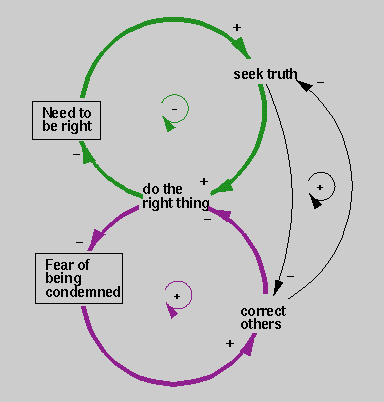
\includegraphics[width=300px]{./media/Type-1-Reformer.png}
\caption{\label{fig:001}Type One Personality - The Perfectionist, The Improver}
\end{figure}

\item Figure 1 Details:
\label{sec:orgdd54a9b}

\begin{itemize}
\item Healthy Loop - colour: Green:
\label{sec:orgee40a78}

\begin{itemize}
\item Green = Controlled by Basic Desire:
\begin{itemize}
\item Need to be right -> seek truth -> do the right thing -> Need to be right
\end{itemize}
\end{itemize}

In the healthy state, the need to be right induces Type Ones to seek truth and do the right thing. When Ones are doing the right thing, the need is satisfied and a balance is reached.

In the average state, when Ones' are not working hard to seek the truth and do the right thing, the need to be right increases, which helps Ones to again work hard to seek the truth. Thus the balancing loop can help Ones to recover.

\item Unhealthy loop - colour: Magenta:
\label{sec:org1d545cb}

\begin{itemize}
\item Magenta = Controlled by Basic Fear:

\begin{itemize}
\item Fear of being condemned -> correct others -> do the right thing -> Fear of being condemned
\end{itemize}
\end{itemize}

In the unhealthy state, the basic fear of being condemned can cause Type Ones to correct and condemn others first as a defense, which is often not the right thing to do, which further increases Ones' basic fear. The cycle continues to build up.

\item Insight:
\label{sec:org6ca0887}
We can see from the diagram that a way to help break the control of the basic fear is to weaken the unhealthy loop. Ones can refrain from correcting others and start examining self for truth, which will help Ones to do the right thing, and reduce the fear of being condemned.
\end{itemize}


\item Detailed Descriptions:
\label{sec:orgc56b0e7}

The Reformer can be a very heroic character...always willing to stand up for what he or she believes in, very aware of what's right and wrong. It's interesting that Ones are hardly ever overweight, which again is that sense of perfection. Their most outstanding character trait is moral courage...but of course they've also got a fatal flaw, like everyone else. (We'll come back to the flaws after the rest of the types and subtypes.)

Perfectionists are realistic, conscientious, and principled. They strive to live up to their high ideals.

\begin{itemize}
\item How to Get Along with Me
\label{sec:org8e32d37}

Take your share of the responsibility so I don't end up with all the work.
Acknowledge my achievements.  I'm hard on myself. Reassure me that I'm fine the way I am. Tell me that you value my advice.  Be fair and considerate, as I am.  Apologize if you have been unthoughtful. It will help me to forgive. Gently encourage me to lighten up and to laugh at myself when I get uptight, but hear my worries first.

\item What I Like About Being a One
\label{sec:orge8895bc}

being self-disciplined and able to accomplish a great deal working hard to make the world a better place having high standards and ethics; not compromising myself being reasonable, responsible, and dedicated in everything I do being able to put facts together, coming to good understandings, and figuring out wise solutions being the best I can be and bringing out the best in other people.

\item What's Hard About Being a One
\label{sec:org6e62eb9}

being disappointed with myself or others when my expectations are not met feeling burdened by too much responsibility thinking that what I do is never good enough not being appreciated for what I do for people being upset because others aren't trying as hard as I am obsessing about what I did or what I should do being tense, anxious, and taking things too seriously.

\item Ones as Children
\label{sec:org18e1db3}

Often criticize themselves in anticipation of criticism from others refrain from doing things that they think might not come out perfect focus on living up to the expectations of their parents and teachers are very responsible; may assume the role of parent hold back negative emotions (``good children aren't angry'')

\item Ones as Parents
\label{sec:orgdd19d18}

Teach their children responsibility and strong moral values are consistent and fair discipline firmly
\end{itemize}
\end{itemize}

\subsubsection*{Type 2 - The Helper, Nurturer:}
\label{sec:org23ad84f}

The Helper, the Giver, who loves taking care of other people and feeling needed. They'll go out of their way to nurture everyone around them, always focusing on what others need more than on what they need. In fact, they'll frequently neglect their own needs and wind up feeling kind of hurt because, ``With all I do for everyone else, what thanks do I get?''       Two's motto is ``People depend on me,'' and they live to be needed. An example might be Beth in Little Women, or Rachel in Susan Elizabeth Phillips' DREAM A LITTLE DREAM, where she was starving herself to feed her little boy. Twos are constantly giving, giving, giving.

\begin{itemize}
\item Key Points:
\label{sec:org02934a4}
\begin{itemize}
\item World View: ``People depend on my help. I am needed''
\item Basic Desire: ``I need to be loved''
\item Basic Fear: ``I am afraid of being unloved''
\end{itemize}

\item Diagram (figure 2):
\label{sec:org4aa6cee}

\begin{figure}[htbp]
\centering
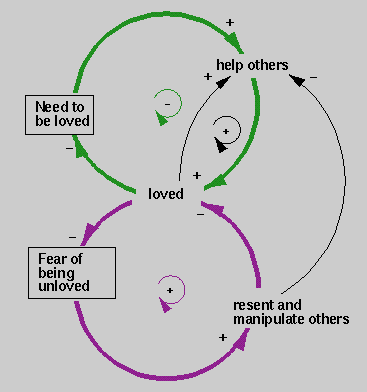
\includegraphics[width=300px]{./media/Type-2-Perfectionist.png}
\caption{\label{fig:002}Type One Personality - The Perfectionist, The Improver}
\end{figure}

\item Figure 2 Details:
\label{sec:orgb6c13cc}

\begin{itemize}
\item Healthy Loop (green) - Controlled by Basic Desires
\label{sec:orga7791aa}

\begin{itemize}
\item Cycle: 
\begin{enumerate}
\item (start cycle) Need to be loved
\item Help others (share the love)
\item Feel the love (from others)
\item (repeat cycle) Need to be loved
\end{enumerate}
\end{itemize}

In the healthy state, the need to be loved induces Type Twos to help others which causes them to be loved. When Twos feel loved, the need is satisfied and a balance is reached.

In the average state, when Twos' are not helping others and are not loved, the need to be loved increases, which helps Twos to again reach out and help others. Thus the balancing loop can help Twos to recover.

\item Unhealthy loop (magenta) - Controlled by Basic Fear
\label{sec:org12ef584}

\begin{itemize}
\item Cycle:
\begin{enumerate}
\item (start cycle) Fear of being unloved
\item Resent and manipulate others
\item Feel the love (from others)
\item (repeat cycle) Fear of being unloved
\end{enumerate}
\end{itemize}

In the unhealthy state, the basic fear of being unloved can cause Type Twos to feel resentful and try to manipulate others into loving them. This can cause people to love them even less, which further increases Twos' basic fear. The cycle continues to build up.

\item Insight:
\label{sec:orgf935c16}

We can see from the diagram that a way to help break the control of the basic fear is to weaken the unhealthy loop. Twos can refrain from manipulating othe
\end{itemize}

\item Detailed Description:
\label{sec:org82804bc}

Yadda, yadda, yadda...

\begin{itemize}
\item How to Get Along with Me
\label{sec:org238d4a9}

Yadda, yadda, yadda...

\item What I Like About Being a YADDA
\label{sec:org996e2eb}

Yadda, yadda, yadda...

\item What's Hard About Being a YADDA
\label{sec:orgf551ff6}

Yadda, yadda, yadda...

\item YADDA as Children
\label{sec:org146c221}

Yadda, yadda, yadda...

\item YADDA as Parents
\label{sec:org7e0a3ff}

Yadda, yadda, yadda...
\end{itemize}
\end{itemize}

\subsubsection*{Type 3 - The Motivator, Achiever:}
\label{sec:org3ce7056}

The Succeeder, the Performer…  These people are very aware of the right image. They're always onstage, projecting whatever the situation requires. Success, career and achievement are important to them...no matter what's going on around them, the Threes will look really, really good. They go around believing (and this is their motto), ``The world values a champion...I must avoid failure.'' So you can imagine the internal conflict when you get a Type Three who's faced with the prospect of failure.

At their worst a Three will embody charm without substance, at their best they embody excellence with a heart. Oprah Winfrey might be a real-life Three; Jay Gatsby might be a fictional one. Threes are often the oldest or only child in their family, because the firstborn is almost always oriented toward being the best and performing the best—and that's what Threes do.

\begin{itemize}
\item Key Points:
\label{sec:orgf6b933a}
\begin{itemize}
\item World View: ``Yadda Yadda Yadda''
\item Basic Desire: ``Yadda Yadda Yadda''
\item Basic Fear: ``Yadda Yadda Yadda''
\end{itemize}

\item Diagram (figure 3):
\label{sec:org9191ef4}

\item Figure 3 Details:
\label{sec:org228ec54}

\begin{itemize}
\item Healthy Loop - colour: Green:
\label{sec:org10fc1d9}

\begin{itemize}
\item Green = Controlled by Basic Desire:
\begin{itemize}
\item 
\end{itemize}
\end{itemize}

In the healthy state, Yadda Yadda Yadda...

\item Unhealthy loop - colour: Magenta:
\label{sec:orged4c93b}

\begin{itemize}
\item Magenta = Controlled by Basic Fear:

\begin{itemize}
\item 
\end{itemize}
\end{itemize}

In the unhealthy state, yadda yadda yadda...

\item Insight:
\label{sec:org26b4179}

Yadda, yadda, yadda...
\end{itemize}

\item Detailed Description:
\label{sec:org0f24727}

Yadda, yadda, yadda...

\begin{itemize}
\item How to Get Along with Me
\label{sec:org67ed92c}

Yadda, yadda, yadda...

\item What I Like About Being a YADDA
\label{sec:orgacc36be}

Yadda, yadda, yadda...

\item What's Hard About Being a YADDA
\label{sec:orgfc3af66}

Yadda, yadda, yadda...

\item YADDA as Children
\label{sec:org59d4566}

Yadda, yadda, yadda...

\item YADDA as Parents
\label{sec:orgb69907a}

Yadda, yadda, yadda...
\end{itemize}
\end{itemize}

\subsubsection*{Type 4 - The Romantic:}
\label{sec:org7894b1f}

The Artist, the Individualist… These are people who love drama and tragedy and falling in love. They have BIG feelings, and they don't like feeling ordinary because that's too flat. Nothing is ever quite grand enough, long enough...they dream about the perfect love, and they're the best at offering wholehearted sympathy when you're feeling low. They make good teachers, actors, counselors, what Tom Condon called ``translators of humanity.''

When I did an enneagram website survey, looking for literary characters who fit each type, I was amazed at the responses for who's a Type Four. Somebody said Scarlett O'Hara, who devoted her whole life to pursuing the love of Ashley—in terms of romantic drive, Scarlett was definitely a Four. Somebody said ALL the Anne Rice characters, because of their huge, vast, sweeping emotions...big ups, big downs.

\begin{itemize}
\item Key Points:
\label{sec:orgf1c3ad7}
\begin{itemize}
\item World View: ``Yadda Yadda Yadda''
\item Basic Desire: ``Yadda Yadda Yadda''
\item Basic Fear: ``Yadda Yadda Yadda''
\end{itemize}

\item Diagram (figure 4):
\label{sec:orgd7b8812}

\item Figure 4 Details:
\label{sec:org30a0f06}

\begin{itemize}
\item Healthy Loop - colour: Green:
\label{sec:org337b44e}

\begin{itemize}
\item Green = Controlled by Basic Desire:
\begin{itemize}
\item 
\end{itemize}
\end{itemize}

In the healthy state, Yadda Yadda Yadda...

\item Unhealthy loop - colour: Magenta:
\label{sec:org37a2ebf}

\begin{itemize}
\item Magenta = Controlled by Basic Fear:

\begin{itemize}
\item 
\end{itemize}
\end{itemize}

In the unhealthy state, yadda yadda yadda...

\item Insight:
\label{sec:orgb3fbe61}

Yadda, yadda, yadda...
\end{itemize}

\item Detailed Description:
\label{sec:orgf12a7ed}

Yadda, yadda, yadda...

\begin{itemize}
\item How to Get Along with Me
\label{sec:orgf269680}

Yadda, yadda, yadda...

\item What I Like About Being a YADDA
\label{sec:orgce59aaa}

Yadda, yadda, yadda...

\item What's Hard About Being a YADDA
\label{sec:org3f2723f}

Yadda, yadda, yadda...

\item YADDA as Children
\label{sec:orga8fdf25}

Yadda, yadda, yadda...

\item YADDA as Parents
\label{sec:org56f349e}

Yadda, yadda, yadda...
\end{itemize}
\end{itemize}

\subsubsection*{Type 5 - The Thinker, Observer:}
\label{sec:org6974b50}

The Thinker, who'd rather be behind a book than out there involved in the world. They like to keep back, keep to themselves, study like crazy but always from a distance. They tend to ``compartmentalize'' their lives: work here, family there, one friend here, another group over there.... They're proud of getting by with very little, and they're very careful about guarding their time and their privacy and their personal space.

Sherlock Holmes sounds like a Five, because he's not involved in the world except on an intellectual level. Real-life Fives might be Albert Einstein (your classic ivory-tower professor), Greta Garbo (``I want to be alone''), and George Lucas (who dreamed up the whole Star Wars universe). Fives are out there in this whole other dimension, and it's mainly a 
world of the mind.

\begin{itemize}
\item Key Points:
\label{sec:org95fa1f5}
\begin{itemize}
\item World View: ``Yadda Yadda Yadda''
\item Basic Desire: ``Yadda Yadda Yadda''
\item Basic Fear: ``Yadda Yadda Yadda''
\end{itemize}

\item Diagram (figure 5):
\label{sec:orgd8484da}

\item Figure 5 Details:
\label{sec:org90765e3}

\begin{itemize}
\item Healthy Loop - colour: Green:
\label{sec:org994e60c}

\begin{itemize}
\item Green = Controlled by Basic Desire:
\begin{itemize}
\item 
\end{itemize}
\end{itemize}

In the healthy state, Yadda Yadda Yadda...

\item Unhealthy loop - colour: Magenta:
\label{sec:orgce88596}

\begin{itemize}
\item Magenta = Controlled by Basic Fear:

\begin{itemize}
\item 
\end{itemize}
\end{itemize}

In the unhealthy state, yadda yadda yadda...

\item Insight:
\label{sec:orgf97b23b}

Yadda, yadda, yadda...
\end{itemize}

\item Detailed Description:
\label{sec:orgb46e49c}

Yadda, yadda, yadda...

\begin{itemize}
\item How to Get Along with Me
\label{sec:org93837bb}

Yadda, yadda, yadda...

\item What I Like About Being a YADDA
\label{sec:orga216e9c}

Yadda, yadda, yadda...

\item What's Hard About Being a YADDA
\label{sec:org549f8e6}

Yadda, yadda, yadda...

\item YADDA as Children
\label{sec:orgbbf6f4d}

Yadda, yadda, yadda...

\item YADDA as Parents
\label{sec:org23eaf71}

Yadda, yadda, yadda...
\end{itemize}
\end{itemize}

\subsubsection*{Type 6 - The Skeptic, Defender:}
\label{sec:org8e0cf3a}

The Trooper… These are the people who get the job done. They're very aware of any possible threat to their well-being or the people they love; they're very aware of the rules and determined to always keep them...or to always break them. (That's the counter-phobic Six, the James Dean rebel type.) Either way, Sixes are very loyal, steady, always on the lookout for danger, good to have on your side.

It's interesting that in America there are more Sixes and Threes than any other type. Threes are flashier, Sixes are more steady and the Six hero is probably more a beta than an alpha male. I remember a Nora Roberts book where the heroine thought the hero didn't love her because as a special present he gave her a set of tires for her car, and a wise observer pointed out that there was PROOF he loved her—he wanted to keep her safe.

\begin{itemize}
\item Key Points:
\label{sec:org752be5c}
\begin{itemize}
\item World View: ``Yadda Yadda Yadda''
\item Basic Desire: ``Yadda Yadda Yadda''
\item Basic Fear: ``Yadda Yadda Yadda''
\end{itemize}

\item Diagram (figure 6):
\label{sec:org913c39b}

\item Figure 1 Details:
\label{sec:orgef64e07}

\begin{itemize}
\item Healthy Loop - colour: Green:
\label{sec:org5ab9607}

\begin{itemize}
\item Green = Controlled by Basic Desire:
\begin{itemize}
\item 
\end{itemize}
\end{itemize}

In the healthy state, Yadda Yadda Yadda...

\item Unhealthy loop - colour: Magenta:
\label{sec:orgc77cd40}

\begin{itemize}
\item Magenta = Controlled by Basic Fear:

\begin{itemize}
\item 
\end{itemize}
\end{itemize}

In the unhealthy state, yadda yadda yadda...

\item Insight:
\label{sec:orgff39017}

Yadda, yadda, yadda...
\end{itemize}

\item Detailed Description:
\label{sec:org428fbf6}

Yadda, yadda, yadda...

\begin{itemize}
\item How to Get Along with Me
\label{sec:orga19895f}

Yadda, yadda, yadda...

\item What I Like About Being a YADDA
\label{sec:org292c55c}

Yadda, yadda, yadda...

\item What's Hard About Being a YADDA
\label{sec:org90547be}

Yadda, yadda, yadda...

\item YADDA as Children
\label{sec:orgf74251e}

Yadda, yadda, yadda...

\item YADDA as Parents
\label{sec:orgc5d65b2}

Yadda, yadda, yadda...
\end{itemize}
\end{itemize}

\subsubsection*{Type 7 - The Enthusiast, Adventurer:}
\label{sec:org8da37d8}

The Enthusiast... They want to keep having new experiences, try whatever there is. They're interested in everything and everybody, at least at first glance, and they love to plan things, plan trips, plan new activities—whether or not they actually carry out those plans. They like to keep all their options open rather than settle for just one of anything.

Sevens are charming as all-get-out...maybe not so good over the long haul, but boy, they're wonderful to have dinner with. When they aren't all mentally healthy and together, it's usually because they've deliberately avoided being alone with themselves. Sevens who let themselves examine their feelings become more realistic, more generous; and they're almost always cheerful, curious and open to new experiences. Either way, they're fascinating to be with—fun, intriguing, delightful people.

\begin{itemize}
\item Key Points:
\label{sec:orgf268656}
\begin{itemize}
\item World View: ``Yadda Yadda Yadda''
\item Basic Desire: ``Yadda Yadda Yadda''
\item Basic Fear: ``Yadda Yadda Yadda''
\end{itemize}

\item Diagram (figure 7):
\label{sec:orga862532}

\item Figure 1 Details:
\label{sec:org23ab512}

\begin{itemize}
\item Healthy Loop - colour: Green:
\label{sec:org70293dc}

\begin{itemize}
\item Green = Controlled by Basic Desire:
\begin{itemize}
\item 
\end{itemize}
\end{itemize}

In the healthy state, Yadda Yadda Yadda...

\item Unhealthy loop - colour: Magenta:
\label{sec:org35aa937}

\begin{itemize}
\item Magenta = Controlled by Basic Fear:

\begin{itemize}
\item 
\end{itemize}
\end{itemize}

In the unhealthy state, yadda yadda yadda...

\item Insight:
\label{sec:orgcd2d59c}

Yadda, yadda, yadda...
\end{itemize}

\item Detailed Description:
\label{sec:org93f9d80}

Yadda, yadda, yadda...

\begin{itemize}
\item How to Get Along with Me
\label{sec:org359489a}

Yadda, yadda, yadda...

\item What I Like About Being a YADDA
\label{sec:org6a83d01}

Yadda, yadda, yadda...

\item What's Hard About Being a YADDA
\label{sec:orgd091a82}

Yadda, yadda, yadda...

\item YADDA as Children
\label{sec:org0f1c589}

Yadda, yadda, yadda...

\item YADDA as Parents
\label{sec:orgeaa1a72}

Yadda, yadda, yadda...
\end{itemize}
\end{itemize}

\subsubsection*{Type 8 - The Leader, Controller:}
\label{sec:org81e5798}

The Aggressor, the Chief… This person is a self-confident, natural leader. They're used to taking charge, getting things done, making sure everyone gets a fair shake. They go after what they want, always keeping an eye out for the people they care about; they're strong individuals who take it upon themselves to defend the weak...kind of a Wild West sheriff mentality.

An Eight's motto is ``I defend the innocent in an unjust world.'' And this is incredibly heroic—except that not everybody agrees on what is innocence and what is justice, so you might have some people who think this Eight is a real jerk! Scarlett O'Hara might be an Eight, considering how she went back to Tara and bossed everybody around and saved them from starvation. Some of the family resented her for it, but she was determined to get her way and make sure everybody at Tara survived...this take-charge attitude is what makes an Eight heroic.

\begin{itemize}
\item Key Points:
\label{sec:org50ae798}
\begin{itemize}
\item World View: ``Yadda Yadda Yadda''
\item Basic Desire: ``Yadda Yadda Yadda''
\item Basic Fear: ``Yadda Yadda Yadda''
\end{itemize}

\item Diagram (figure 8):
\label{sec:org831d1a8}

\item Figure 8 Details:
\label{sec:org730c225}

\begin{itemize}
\item Healthy Loop - colour: Green:
\label{sec:org3539e1c}

\begin{itemize}
\item Green = Controlled by Basic Desire:
\begin{itemize}
\item 
\end{itemize}
\end{itemize}

In the healthy state, Yadda Yadda Yadda...

\item Unhealthy loop - colour: Magenta:
\label{sec:orgb1bcf71}

\begin{itemize}
\item Magenta = Controlled by Basic Fear:

\begin{itemize}
\item 
\end{itemize}
\end{itemize}

In the unhealthy state, yadda yadda yadda...

\item Insight:
\label{sec:org4ec16f4}

Yadda, yadda, yadda...
\end{itemize}

\item Detailed Description:
\label{sec:org7b65c90}

Yadda, yadda, yadda...

\begin{itemize}
\item How to Get Along with Me
\label{sec:orga25f8f4}

Yadda, yadda, yadda...

\item What I Like About Being a YADDA
\label{sec:orgb40fe09}

Yadda, yadda, yadda...

\item What's Hard About Being a YADDA
\label{sec:orga9873e9}

Yadda, yadda, yadda...

\item YADDA as Children
\label{sec:org08fa2c1}

Yadda, yadda, yadda...

\item YADDA as Parents
\label{sec:orgd04055f}

Yadda, yadda, yadda...
\end{itemize}
\end{itemize}

\subsubsection*{Type 9 - The Peacemaker:}
\label{sec:orgb640c46}

The Mediator.  Peacemakers want everyone to get along and everything to be nice. They don't like conflict; they don't like having to pick sides...even picking chocolate or vanilla. They tend to go along with the flow, whatever that might be, and instead of exploring their own preferences, they kick back with TV or food or whatever's comfortable. There's usually some anger back there, but it's completely denied. Nines are excellent at ignoring their own feelings.

They're the ones who'll be just kind of sitting back, letting everybody else flap around them. A few years ago there was a survey as to what types are most attractive to other types, and more women want to marry a Nine than any other type of man. (More men want to marry a Two.)

\begin{itemize}
\item Key Points:
\label{sec:orgde54a83}
\begin{itemize}
\item World View: ``Yadda Yadda Yadda''
\item Basic Desire: ``Yadda Yadda Yadda''
\item Basic Fear: ``Yadda Yadda Yadda''
\end{itemize}

\item Diagram (figure 9):
\label{sec:orga7aa542}

\item Figure 1 Details:
\label{sec:orged925aa}

\begin{itemize}
\item Healthy Loop - colour: Green:
\label{sec:orga7c45f9}

\begin{itemize}
\item Green = Controlled by Basic Desire:
\begin{itemize}
\item 
\end{itemize}
\end{itemize}

In the healthy state, Yadda Yadda Yadda...

\item Unhealthy loop - colour: Magenta:
\label{sec:org3b0debe}

\begin{itemize}
\item Magenta = Controlled by Basic Fear:

\begin{itemize}
\item 
\end{itemize}
\end{itemize}

In the unhealthy state, yadda yadda yadda...

\item Insight:
\label{sec:org90e59ae}

Yadda, yadda, yadda...
\end{itemize}

\item Detailed Description:
\label{sec:orgb81b4b9}

Yadda, yadda, yadda...

\begin{itemize}
\item How to Get Along with Me
\label{sec:org2ed19b4}

Yadda, yadda, yadda...

\item What I Like About Being a YADDA
\label{sec:orge1b62ac}

Yadda, yadda, yadda...

\item What's Hard About Being a YADDA
\label{sec:orge58f867}

Yadda, yadda, yadda...

\item YADDA as Children
\label{sec:orgd35d62c}

Yadda, yadda, yadda...

\item YADDA as Parents
\label{sec:orgc59c70e}

Yadda, yadda, yadda...
\end{itemize}
\end{itemize}

\subsubsection*{Summary:}
\label{sec:org067980c}

From the short examples of all the types above, it’s easy to see how each of them has good and bad traits.  Each type has innately wonderful traits, which, taken to excess, can be bad.  This is a good thing, because we need some conflict between our perfectly wonderful heroes and heroines!

\subsubsection*{SubTypes:}
\label{sec:org439e46e}

If you met Sherlock Holmes and Greta Garbo in an online chat loop, you wouldn't have any trouble telling them apart. They're both Fives, yes, but no two matching enneagram types are alike anymore than two matching astrological types are alike.

One reason is because of the subtypes: Self-preservation, Intimacy, and Social. Everyone values each of these in different amounts. When you're holed up studying for the final exam, that's self-preservation. When you're on a dinner date talking for hours, that's intimacy. And when you're in a crowd of fans all cheering for the home team, that's social. We all do all three.

Ideally you have them all weighted equally in your life, but most of us tend to hang out more in one area than in the others. And of course that area is going to be a source of great strength because we're good at it, and it's also going to be a source of great weakness because we've left the others alone. But great weakness is a fine thing when it comes to creating characters! So see which subtype sounds like your hero or heroine (or yourself and your real-life hero).

\begin{itemize}
\item The Self-Preservation subtype:
\label{sec:org12bbb94}

This person is concerned with exactly that: self-preservation. Does their household have enough water to last through a nuclear winter? How are they gonna pay their kid's tuition? Is there anywhere they can get some privacy? Where can they find their favorite kind of soda? These people are concerned with basic survival issues, survival of the body or the spirit or both. If they were stranded on a desert island with plenty of survival gear, they'd be fine by themselves.

Now, how—in a romance—can this self-preservation trait work? It's not what you'd expect from a typical romance character, right? An adventure thriller, yes, you want your hero or heroine to save the sinking boat and elude the Nazis...but on an emotional level, this self-preservation can be a wonderful character trait for building internal conflict. Imagine someone who's trying to preserve their well-being, their sanity, their heart, by not falling in love. Imagine the tension as they find themselves falling in love, and resisting, and falling, and resisting.... Self-preservation is a great trait for a romance novel character!

\item The intimacy-subtype:
\label{sec:org57ea9fc}

This person is someone who's concerned with one-on-one relationships. Not just their lover, but every individual friendship. They want to spend time alone with everyone they care about, just the two of them, talking as intimately as they can: ``What's going on? How're you feeling? Here's what's new with me.'' If they were on that desert island, they'd want one other person with them. Just one...who'd be just as involved with the relationship as they are.

Now it's no good for a romance if your hero and heroine are both intimacy subtypes who wants the same intimacy at the same time, because then all you have is two people kissing and holding hands for chapter after chapter. But suppose one character wants this intimacy with not ONLY the lover, but also with the friend next door and the brother across town and the boss and the waitress and the lover's grandmother...there's going to be some conflict, right? I remember a great book where the hero was a social worker who gave himself wholeheartedly to the individual kids at his youth shelter that needed one-on-one contact, and when it came time for the romantic dinner with the heroine while a kid is in crisis...okay, more conflict. So you can see how an intimacy character is great for a romance novel!

\item The Social subtype:
\label{sec:org906809d}

This person is concerned with the community as a whole. They're not so much interested in what's going on within themselves, or what's going on within a particular person, as they are with what's going on in the whole group. That group might be their church, their co-workers, their RWA chapter...whatever it is, these people love being part of the group. They want their entire gang on that desert island, and they want to do their part for the whole group...for the whole social structure.

Already you can see the conflict for a romance novel, right? My dad is a social person, while my mom is an intimacy person, and they've been married for forty-some years. But on Tuesday nights, when she wants him to go with her to ballroom dancing class, and he wants her to go with him to the church prayer group.... Conflict.

Keep in mind that none of the 3 subtypes above is better or worse than any others. Everybody needs to be concerned with the Me, the We Two and the All Of Us in order to have a truly well-balanced life. But there can be conflict between WHATEVER subtypes your characters are, and (fortunately for us writers) that conflict leaves room for growth. Because growth has to happen for these people to reach their happy ending!

Growth can come in two ways. One is that the couple can learn to compromise (like my mom and dad, who agreed they'd spend six Tuesdays at dance class and then the next six Tuesdays at prayer group.) The other way is that they can each overcome something within themselves...and that's fascinating to watch because it gives the reader something to root for in addition to the happily-ever-after.

However, this kind of individual growth can't happen unless a person has something they need to overcome. They need some fatal flaw to be interesting, and we need our characters to overcome something to deserve the happy ending.
\end{itemize}

\subsubsection*{Fatal Flaws:}
\label{sec:org3230275}

It's easy to find ideas for the fatal flaws our characters will have to overcome, because 
the enneagram theorists say that each of the nine types has a deadly sin within them. Although the math is off, because there are seven deadly sins and nine enneagram types, so they made up two more sins which fit the types.

\begin{itemize}
\item ONE's fatal flaw is Anger
\label{sec:orgf8104d9}

These are the perfectionists who get angry when they or anyone else doesn't strive for perfection. Picture a hero whose life has been about upholding what's right and good, maintaining the highest possible standards for himself and everyone around him, being kind of righteous about it and fuming when people don't live up to his standards of perfection—being especially upset when he doesn't live up to his OWN standards of perfection. He's going to be angry at himself when that happens, and of course it's going to happen. So you'll get this wonderful growth as the hero realizes (maybe with some help from the heroine, maybe on his own) that he has to let go of this anger and be more tolerant, more forgiving of the imperfection that's in himself and in everyone else.

\item TWO's deadly sin is Pride
\label{sec:org4d5b6fd}

These are the nurturers who take pride in being indispensable to those people they care for. So far every heroine I've done has been a Two, and every one of them has had to face that truth. She's had to quit knocking herself out trying to create the perfect world for her loved ones. And while this woman who spends her every waking hour nurturing others might sound like a doormat on the surface, in fact she can be a tremendously powerful character to watch. Seeing her overcome that pride in being indispensable, watching her realize that she can let go and the world won't come to an end, is a huge triumph. When she can finally stop doing for others as a way of fitting in, she's discovering her true power...and from then on, her nurturing comes from the strength of love rather than the weakness of pride.

\item THREE's fatal flaw is Deception
\label{sec:orgc0e67ae}

These are the performers who put on a front for the world and for themselves in order to look just right. This person will have to overcome the habit of deception...to quit putting on a perfect face and discover his or her true self. Imagine the impact of someone coming to realize that his or her whole life has been a series of performances, of trying to be the best at whatever comes up, of doing whatever will present the best facade to the public—and for the first time actually looking at what's really inside him or herself. This is a great chance for the lover to help out, to help this person discover that they can be loved for themselves...that they don't need a perfect facade in front of everyone in the world. That's a wonderful road to a happy ending for the Three.

\item FOUR's deadly sin is Envy
\label{sec:org18c2a0b}

These are the romantics who feel like everyone else in the world has a more rich and satisfying life. They'll have to let go of envy and appreciate that what they've got is pretty darned good—and this is hard for the Four. Someone whose life is about drama and tragedy and falling in love doesn't WANT to give up all those big up-and-down sweeps, all the glory and pathos and angst and feeling. But what's wonderful is that they don't have to! They can still have that larger-than-life, creative, artistic flair...as long as they let go of the self-pity. Again, this can be with the help of someone who loves them. This someone can show them how to laugh at themselves and the world around them, bring them down to earth while still letting them fly high with their own creative passion.... Watching a Four come to appreciate what they've got in their life can be a joyous, sparkling thing.

\item FIVEs need to overcome Avarice
\label{sec:orga515a1d}

These are the observers who are greedy about their precious time and their own personal space. In order to overcome their deadly sin, they'll have to quit being greedy about their own private selves and learn to share. Someone who spends their whole life wrapped up in solitude will have a really hard time letting a lover into their world. You're going to get some pretty intense conflict and crackling tension as this unfolds. Picture an ivory-tower professor leaving his library door open a crack when the heroine is nearby. Then slamming it shut. Opening it another crack... Picture someone who never talks about their feelings, opening up to a lover for the first time. It's exhilarating, watching a Five realize they can share their private world with someone else...that they can finally open the door and let love in.

\item SIX's fatal flaw is Fear
\label{sec:org25030e0}

These are the defenders who are always aware of possible dangers and worrying about how to handle them. The Six will have to let go of fear and realize you can't always guarantee absolute security. You can imagine a character who lives in fear, right? Not so much a woman-in-jeopardy heroine, afraid of the dark baron up in the Gothic tower, but someone who's driven by the quest for security. It could be financial security, it could be emotional security, but whatever it is, this fear keeps them from living life to the fullest. And now here you have the lover offering a new kind of life...and the Six hesitating, afraid of taking any kind of risk. ``What, jeopardize my comfortable life and the security of my heart to fall in love? I can't do that.'' But for the right love they CAN risk it, and when they do, it's wonderful to watch the payoff.

\item SEVEN's deadly sin is Gluttony
\label{sec:org5ef46d7}

These are the adventurers who want every possible new experience, one right after another. Here's someone who'll have to learn that permanent freedom isn't so great; commitment has its own rewards. And you can imagine the struggle they'll go through to avoid learning this lesson. You've got a character who's the life of the party, ready to go anywhere anytime...and now all of a sudden they're in a situation where they have to slow down, move beyond the good-time surface and really come face to face, heart to heart, with another person. They're gonna resist that with everything they've got—stay out later, party harder, run away to some other distraction—and yet suddenly, this freedom isn't so attractive unless the loved one is part of their life. But only when they make the commitment to love will they realize that now, finally, this is what they've been missing...what they've been searching for all along.

\item EIGHT's fatal flaw is Lust
\label{sec:org1605859}

These are the leaders who lust for power, to be in control, to run the show and get things done their way. This person has to step back and share control, to let go of that lust for power. Here's someone who's spent their whole life running the show, making things happen, getting things done their way, and all of a sudden somebody's expecting them to give up control? Most types wouldn't have much problem sharing control with someone they love, but Eights didn't get to where they are by compromising on anything. So they resist. And maybe the lover walks away. And they try everything they CAN to win back this person—they want to give the lover everything, but they want to do it their way—and only after they give up this lust for being in control will they realize that here's the key to a kind of success they've never known before.

\item NINE's fatal flaw is Sloth
\label{sec:org2d1ea67}

These are the peacemakers who want to just sit back and have everything be nice and comfortable. This person is gonna have to give up the comfort of neutrality and make some kind of a stand. Here they've has spent a lifetime taking things easy, not getting worked up one way or another, refusing to take action, refusing to get involved on either side of anything. Now here they're faced with having to come down on one side or another...they're gonna have to declare themselves: this is what I want, this is what I believe, this is who I am, take it or leave it. (And maybe in a romance they're worried that the lover will leave it.) They've never let that happen before, they've never put themselves in a position where they have to take a stand...but now they HAVE to take some kind of action, make a stand for something, and it'll open their eyes to a whole new way of living.

\item Summary:
\label{sec:org5ba368e}

So you can see how all nine types have their own deadly sin. And you can see how, even with these fatal flaws, none of these people is a jerk. Each of them is someone we can sympathize with and root for, because they're ALL people with tremendous potential to learn and grow and change. And because all nine of these deadly sins can be overcome, the readers can put the book down satisfied: ``Ah, another happy ending.''

Each one of us could sit down and write nine books where the heroes and heroines learn those nine things—overcoming anger with tolerance, pride with relinquishment, deception with honesty, envy with appreciation, avarice with sharing, fear with risk, gluttony with commitment, lust with compromise and sloth with action—and you can bet that we'd each come up with a different happy ending. But even those nine lessons aren't the best part of enneagram theory. Its greatest value for writers is in letting the personality types, subtypes and fatal flaws inspire ideas...which is the whole fun of romance writing.

I wish that kind of fun for each of us, and I'll look forward to reading how all our characters overcome their fatal flaws!
\end{itemize}

\subsection{Enneagram Type Tests:}
\label{sec:org579b1fe}
\subsubsection*{Introduction \& Example Tests:}
\label{sec:orgdb2df61}

If you are super serious about doing this, you must purchase the official tests

Take the quick (less accurate) on-line tests here:

\begin{itemize}
\item The New Test: \url{http://9types.com/newtest/index.php}
\item The RHETI Test: \url{http://9types.com/rheti/index.php}
\end{itemize}

When I first learned about this test a few years ago I took the test then and my results were as follows:

\begin{center}
\begin{tabular}{rrrrrrrrr}
\hline
Type 1 & Type 2 & Type 3 & Type 4 & Type 5 & Type 6 & Type 7 & Type 8 & Type 9\\
\hline
5 & 4 & 5 & 4 & 5 & 2 & 7 & 0 & 4\\
\hline
\end{tabular}
\end{center}

The highest score indicated my basic personality was type 7.  At that time I also leaned a bit towards Type 1, Type 3, and Type 5.  My antithesis types were: Type 8 and Type 6.  My neutral types were: Type 2, Type 4, and Type 9.

This was my very first test before knowing anything about the enneagram types!  The rest of the tests below are time stamped headings in descending chronological order (most recent on top)

You can take these tests for yourself, but most importantly as a tool to dive deep into the personalities of the characters in your stories... To do this, you must become a shaman able to shift into your character's mind and be that person completely, as if your character is the one sitting on that comfy chair in the analyst's office... Not you! To do this, you must be more than an actor.. you need to actually become that person for the duration of the test!  Your character's responce to the questions will be totally different than if you were taking the test!  How does it feel being that person? lol

\begin{itemize}
\item Test Results on: \textit{<2020-06-09 Tue>}
\label{sec:org7c3b40b}

\begin{center}
\begin{tabular}{rrrrrrrrr}
\hline
Type 1 & Type 2 & Type 3 & Type 4 & Type 5 & Type 6 & Type 7 & Type 8 & Type 9\\
\hline
0 & 1 & -2 & 6 & 3 & 1 & 3 & -5 & -7\\
\hline
\end{tabular}
\end{center}

\item Test Results on: \textit{<2016-04-24 Sun>}
\label{sec:org849f682}

I took the test again today almost a whole year later…  Results were much different!
My basic personality is: Type 4 ``the intuitive reserved artist''.  My subtype is Type 5 ``The Observer''.

My antithesis types are: 1, 9, \& 2.  My neutral types are: 3, 6, 7 \& 8.

\begin{center}
\begin{tabular}{rrrrrrrrr}
\hline
Type 1 & Type 2 & Type 3 & Type 4 & Type 5 & Type 6 & Type 7 & Type 8 & Type 9\\
\hline
-5 & -2 & 0 & 6 & 3 & 0 & 0 & 1 & -3\\
\hline
\end{tabular}
\end{center}

As you can see… my current journey into fulfilling my life long dream of producing music and art full time has gotten me much more reclusive and focused on making that happen over the past year!!!
\end{itemize}

\chapter{Audio Drama \emph{(guide)}}
\label{sec:orgd0abc48}
\section{How to Write Radio Drama Cues}
\label{sec:orgee093c2}
\subsection{Introduction:}
\label{sec:org99b4219}
This guide started out as an adaptation of Tony Palermo's ``How to Write Radio Drama Cues'' and the methods he teaches on his website: \url{https://www.ruyasonic.com/}, (adapted for Emacs Org-Mode and Fountain Screenwriting mode). Over time, many things ended up being formatted differently from Tony's examples to conform with Fountain syntax (which is biased towards standard film screenwriting styles). 

It did not take long for me to get frustrated with that.  I embarked on a quest to find a way to tweak Fountain to better translate into proper Radio Drama format as Tony Palermo Teaches it. (good luck with that) But guess what...  I laboured over that for a while and finally got something working pretty nicely now! (thanks to the Python programming language, and the flexibility of Fountain mode's ``power user'' tricks).

Harmonic Alchemy Modular Emacs configures Fountain screenplay scrips using a Python script called: ``Afterwriting'' to prepare much of the front matter programmatically for you. Page Headings and Footers are set up this way so you don't need to go through the labour of putting them directly within your scripts after each page break (which changes every time you edit your scripts! OMG!  Here, your page headings and footers will automagically appear at the top and bottom of each page (whereever that page break may occur, and they will keep track of where page breaks occur automagically as well)...

Scripts displayed within the editor look differently than they do in the final printout.. This is normal and a good thing, as the needs of the writer/editor are different than the needs of the performers...

Tony's Radio Adaptation of Frank Capra's classic film, “It’s a Wonderful Life” is used in this guide for the example cues below... All credit for any reprinted material within this guide go to: \href{https://www.ruyasonic.com/tpalermo.htm}{Tony ``SPARX'' Palermo}.

Much of the intro material curated below has not changed much from \href{https://www.ruyasonic.com/wrt\_cues.htm}{Tony's original article which can be found here}... It is not my intention to change anything that Tony teaches, however in order to make his wisdom accessable to users of Fountain Screenwriting software (adapted to work with Tony's Radio Drama Cues Formting styles) I had to write this guide and import much of his instruction into it...

I strongly encourage you to visit \href{https://www.ruyasonic.com/}{ALL of Tony Palermo's RuyaSonic Website} to get a much better education on the entire Radio Drama Process (e.g., prepairing and writing scripts, pre-production, production, post-production, sound-cues, music, etc...) 

The information contained within this guide only focuses on one particular aspect of what you can learn from the above links.  This project is to be used as a template (or cheatsheet) to facilitate the process of creating headings, cues, etc. within Emacs org-mode and fountain-mode, and also to provide easy ways of exporting your scripts to printable PDF files in a format that Tony would approve of. (I hope ;-) 

For a total education on all aspects of Radio Drama with a good perspective on the history of the entire industry, you are strongly encouraged to visit Tony's webpages above!

\subsubsection*{More Info:}
\label{sec:org3eb0e5a}
According to Tony Palermo: ``While there are hundreds of books on writing film screenplays and stage plays, radio scripting isn't a widely known form. (and Fountain Screenwriting Software is not exempt from this ignorance) However, because radio is produced with the script in hand, it is important that the various cues for dialogue, music, and sound effects be able to quickly and clearly communicate the writer's intentions to the cast and crew for rehearsals and performance.''

Below are some of Tony's suggestions and examples to encourage clearly written radio drama scripts.

Through years of radio-drama production experience, Tony found out rehearsals and performances go more smoothly if the scripts are very precise in their instructions to cast and crew.  This Guide addresses those many radio drama conventions and guidelines in an effort to aid writers and directors, (especially those with little radio production experience).

Tony's instructions focus mostly on the concept of ``live production'', where the dialogue, music, and sound effects occur in real time as the program is being performed for stage, recording, or broadcast. Instructions within this guide are focused on post-production sound-design, background music, final mix, mastering etc.  Keep that in mind as you study this guide and compare it with things you may learn on Tony's website...  

Live productions are outside the scope of this guide but I may end up writing another guide about that once I have some experience doing it under my belt... Smaller scale ``live productions'' can be made using my self-designed Stereo Pair Microphone array built from a styrofoam bust (the kind you see used to display hats or head fashions in store windows) with AT4022 matched stereo pair omnidirectional condenser microphones mounted (with microphone heads located where ears would normally be)... A DIY microphone array that costs hundreds of dollars less than a professionally made one, but works just as well.  Maybe even better...  I created a remote recording rig using this array and a Fostex portable digital recorder (also much cheaper than the expensive pro remote digital recorders but sounds almost identical in quality)... Note: the smaller hand held portable recorders (with built in microphones) are not good enough for pro work.  Live performances can be done this way remotely (without needing external power) within any type of acoustic environment...  

These guidelines will aid you greatly if you intend to record dialogue separately and then assemble the finished program in post-production. The intention of writing good radio drama cues is to clearly communicate all instructions, thereby cutting down on misunderstandings, notes, mistakes, and time. A well-written script will save everybody headaches and make your shows easier and cheaper to produce.

Getting used to working with Fountain will take a bit of study... The \href{https://fountain.io/syntax}{Official Fountain Syntax Reference can be found Here}... In addition, Getting help with Emacs Fountain-Mode (after consluting Emacs help with ``C-h m'' from any fountain-mode buffer) can be found directly on the \href{https://github.com/rnkn/fountain-mode}{Fountain-Mode Github Page}... The Most helpful resource however is simply typing ``C-h m'' and reading those docs... 

Fountain-Mode depends on other Emacs Packages to do much of the heavy lifting work... You may find the help you are looking for from those required packages.  The packages Fountain Mode uses are listed on the Fountain-Mode Github Page Link above...

Learning to use Fountain-Mode is pretty straight forward however... Most of your needs will be learning Fountain itself... which IS well documented...

In addition to this guide, you may wish to download some of the short professional free demo scripts \href{https://www.ruyasonic.com/em\_scripts.htm}{offered here on Tony's website}...  Note there are also full scripts available on that link as well.  Also, you can find \href{http://www.genericradio.com/}{more scripts of classic Radio Drama here}... Make sure any scripts you look at were formatted for Radio... Not the Visual dramatic arts... Check to see if it looks or conforms to standards that Tony Recommends...


\subsection{Page Headings:}
\label{sec:orgefe2f92}
\subsubsection*{Introduction:}
\label{sec:orgda3571b}

The purpose of page headings is to indicate what program or episode you're working on and what page you are on in the script. These go across the top of the page.

The examples below would not be typed into your scripts... Instead you will be putting those inside a file called awc-config.json  In the examples below they appear approximately how they would look like in the final print or PDF (with any Fountain formatting marks removed)

Note: within your actual scripts, (not the examples below) Page headings and footers have been automatically configured to show up in the exported PDF and printed pages the way Tony Palermo recommends \href{https://www.ruyasonic.com/wrt\_cues.htm\#CUES}{in this article}.  I chose one of his examples that I liked best from his page on that subject, and configured the script to make sure it gets formatted that way. That configuration happens within an input data file that can be edited to make your page headings and footers look like one of Tony's other ``acceptable examples''.

Before starting a new Radio or Audio Drama script you will need to open a ``data file'' called: awc-config.json (see example below), and ``fill in the blanks'' with your story particulars... As you can see in the example, things are pretty self evident.  

awc-config.json (awc stands for Afterwriting Config) is a ``human readable data file'' but it is also read by a machine that expects things to be in a particular place etc. As you can see there are no instructions (or comments) within the file itself.. Those things are not allowed within .json files. Only text data to be read by a program is allowed.  Don't move any of the lines within this file around... 

You will be replacing one or more things on the right side of the colons ``:'', (e.g., true to false, or visa-versa, the text on right side within quotes after ``print\_footer'': and after ``HEADER'':, ``TITLE'':, ``EPISODE'':, etc...)

Do not change any of the keywords on the left side of the colons ``:''.  That will cause an error! Do not change any word prefixed with a dollar sign ``\$'' anywhere in the file.  Those are also special keywords (like \$TITLE which gets replaced with your specific title text set in another part of the file. You may change the spacing between those \$KEYWORDS however to get the line looking right on the final printed page or PDF. You will have to experiment with that spacing depending on the length of your actual title etc.

If you change your details this way without messing with anything else in the file you will be fine. 

\begin{itemize}
\item Note: Using double asterisks ``\textbf{**}'' below to bracket (delimit) any of the text you are changing (within quoted text sections) will make it BOLD on the exported printed page...  Using a single asterisk ``*'' to delimit text will make it italic on the exported printed page...
\end{itemize}

Unfortunately I have not figured out a way to automatically double-space dialog lines using Fountain Mode... But I am determined to get that working as well... ``Stay tuned... Don't Touch That Dial'' LOL

\begin{itemize}
\item awc-config.json example:
\label{sec:orgab45226}

\lstset{language=js,label= ,caption= ,captionpos=b,numbers=none}
\begin{lstlisting}
{
    "embolden_scene_headers": true,
    "show_page_numbers": true,
    "split_dialogue": true,
    "print_title_page": true,
    "print_profile": "usletter",
    "double_space_between_scenes": false,
    "print_sections": false,
    "print_synopsis": true,
    "print_actions": true,
    "print_headers": true,
    "print_dialogues": true,
    "number_sections": false,
    "use_dual_dialogue": true,
    "print_notes": false,
    "print_footer": "Harmonic Alchemy Productions - siren1@HarmonicAlchemy.productions",
    "print_watermark": "PRODUCTION DRAFT COPY",
    "scenes_numbers": "both",
    "each_scene_on_new_page": true,
    "print_header": "The Lighthouse          Episode S1-001",
    "snippets": {
        "HEADER": "$TITLE          $EPISODE",
        "TITLE": "**The Lighthouse**",
        "EPISODE": "S1-001",
        "CREDIT": "*An Emergent Anomalies - Paranormal Audio Drama*",
        "AUTHOR": "by **Alisha Awen**",
        "DRAFT_DATE": "PRODUCTION SCRIPT"
    }
}
\end{lstlisting}

Once you have changed the meta data within the file as above to fit with your project's particulars, you will be all set to start editing your: ``my-new-screenplay.fountain'' file within an Emacs editor buffer...

\begin{itemize}
\item Note: All fountain screenplay files have a boilerplate section at the top that you don't have to edit ever again (once you do it the first time) That header section is where all the data from the above awc-config.json file gets populated during export.  You will only be changing the Contact: info, the Copyright: info and optionally Tags: or you can remove the Tags: part if you wish...  Once this is edited save your screenplay.fountain to be used as a template for future Radion Drama projects.  You will never again have to edit the boilerplate sections at the top of your scripts after that...
\end{itemize}

\item Important NOTE:
\label{sec:org6e07a17}

I use Fountain source code blocks within the examples below, which displays them in the proper screenplay format (within this org file)... In the case of Page Headings and Footers the examples below use Fountain's general purpose ``Action'' element to get then to look approximately the way they should look on a printed page. Headings are supposed to be set bold face.  In fountain delimiting (bracketing) with two asterisks ``**'' emboldens the text, both in the editor and on the final exported output... You will NOT be doing it this way within your scripts... I only did it this way below for this guide only, to approximate what Tony Palermo instructs us to do with page headings, but understand, my Fountain to PDF Python script takes care of Page Headings and footers. I will say again... You will NOT be putting them into your script directly! Page Headings appear below purely for pedagogical reasons.
\end{itemize}

\subsubsection*{Examples:}
\label{sec:org9e06b6a}

\begin{itemize}
\item Note: Double ``\textbf{**}'' bracketing lines below in examples does not show on the printed pages.  It tells Fountain to embolden the text...  You see it bold in the editor (with the ``\textbf{**}'') You will later see it bold (without the ``**'') on the final printed pages... However, as I said in the introduction above you will not need to type these headings into your scripts directly... Instead, you put them into: awc-config.json as explained above in the Introduction...
\end{itemize}

\lstset{language=fountain,label= ,caption= ,captionpos=b,numbers=none}
\begin{lstlisting}

**Life's Little Ups & Downs            Episode #1829                        10.**

**The Innocents Abroad                                                     -17-**

**Holiday Playhouse       Charles Dickens' A Christmas Carol        REVISED 49.**

**Holiday Playhouse   Charles Dickens' A Christmas Carol     REVISED 49. 7/7/05**

**Holiday Playhouse           Charles Dickens' A Christmas Carol          49-A.**

**Suspense                    Roma Wine Ad                       COMMERCIALS-1.**

\end{lstlisting}

\begin{itemize}
\item Explanation: 
(in Tony's own words)
\label{sec:orgd37e6d6}

The page number should be in the TOP, RIGHT HAND CORNER, so actors can easily see it as they page through their scripts in rehearsal and performance.

\texttt{NOTE:} \textbf{Do NOT put the page number at the bottom of a page}... That only
      slows down tech crew and cast from paging through the script
      to get to a specific page.

Old time radio scripts would use a period after the page number (10. 47. 78.) or put dashes to either side of it (-4- -23- -108-).

Include program and episode titles on your script in case somebody drops their script pages in a production featuring several sketches or commercials. Many troupes don't use staples to hold their scripts together, so pages can get out of order. (I use one staple in the top left corner and instruct my actors on how to turn script pages quietly--slowly flip the page over. Don't ruffle the paper and make a sound.)

If a script page is revised after the printed scripts have been given to cast and crew, indicate REVISED on the new page, so they can substitute the new pages for the old ones. You may also want to add a date, in case there are future revisions. New pages inserted into a script after printing can be designated by adding a letter after the page number. So the paging might go 48, 49, 49-A, 49-B, 50, 51, etc.

For drop-in ads or announcements, I suggest creating separate pages with their own numbering scheme. This way they can be altered or added at the last minute and not affect the page numbering scheme of the dramatic script. All spacing is up to you. For these headings, use a small plain font (like 8-point Arial) and give the page heading a bit of space separating it from the script text so actors won't get confused as they turn to a new page and begin speaking their lines.
\end{itemize}

\subsection{Page Footers:}
\label{sec:orgfc2d7c3}
Everything I said above about page headings also applies to Page Footers as well, (i.e., you will not be typing these into your scripts directly).  Instead you put them into a data file called ``awc-config.json'' which gets read in during the export process... The examples below are shown formatted as best as possible here for pedagogical purposes only...

Footers at the bottom of the page can be used to indicate the production company, the writer's contact info, or to display the date or revision number of the script. Make sure there's sufficient space between the script text and the footer. Again a small 8-point Arial font here will help differentiate the footer from the scripted cues.

\subsubsection*{Typical Footer Examples:}
\label{sec:org7c41146}

\lstset{language=fountain,label= ,caption= ,captionpos=b,numbers=none}
\begin{lstlisting}

        **Production Co. Name 12345 Main St. Radio City CA 90019 - email@something.com**

-- or --

                                  **Fourth Draft 3-04-2003**

\end{lstlisting}

\subsection{Scene Headings:}
\label{sec:org612b0cb}
\subsubsection*{Introduction:}
\label{sec:orgcd592a5}

Radio scene headings are based upon standard Hollywood film screenplay format. They indicate the scene number, description of the scene's location, and time of day. You can also include info such as (FLASHBACK) or (MONTAGE).

A scene is some dramatic action that takes place somewhere.

If one scene ends and then there is a narrator who leads you into another scene, put that narrator's cues in the middle--between the two scenes.

\subsubsection*{Fountain Syntax for RuyaSonic Scene Headings:}
\label{sec:org7574f3e}

Using fountain-mode in Emacs to edit drama scripts is, for the most part, a natural flowing typing experience.  You don't have to indent lines etc... Just start typing your script from the first column, and drama script elements will automagically be detected by fountain-mode (as you type) and, (for most cases) will properly indent and re-display the text as expected, in a way that makes it easy to read within the editor, (just as it would look in the final print version) but also using colours to further distinguish different elements within the script.

For the cases where fountain-mode cannot decide what to do, or tries to format a line to conform to a different script element, (e.g, a dialog cue when you wanted a sound cue, etc.) there are a few power user tricks you can employ to train fountain-mode to do what you intend it to do...

In the case of Scene Headings, Fountain detects these fine if they start with something like: INT or EXT etc. and are followed by a blank line...  Some of the examples Tony gives in his Instructions may not be detected by fountain automagically. For those ambiguous cases Fountain provides a ``power user'' trick.  Simply start any scene heading with a period ``.'' (full stop) character. That will signal fountain-mode to force Fountain to take the line as a Scene Heading...

I use Fountain source code blocks within the examples below. The Org-Babel package in turn displays the contents of those source code blocks formatted exactly as they would appear within a normal Emacs buffer window visiting a ``screenplay.fountain'' file using fountain-mode.

Notice the scene headings within the examples below where a period ``.'' (full stop) character has been placed at the beginning of the line.  This signals Fountain Mode to force the line into a Scene Heading...

If you write your scripts as shown in the examples below, the print versions will confirm exactly to Tony Palermo's guidelines. (i.e., They will be displayed in a 12-point New Courier Font that has been bolded to photocopy better).

According to Tony Palermo's guidelines, All cues for dialogue, music and sound effects within a radio drama script need to be double-spaced, to allow for easy reading on the fly and notes or new lines added in rehearsal. To make Fountain conform to this rule, keep your dialog lines short (don't continue them on to full 80 or more columns) and force double spacing of the next line by hitting carrage return once, entering two space characters, and then hitting the carrage return a second time... (just like in the old days on a manual typewriter ;-)

\subsubsection*{Examples:}
\label{sec:org25afe20}

Radio scene headings are based upon standard Hollywood film screenplay format. They indicate the scene number, description of the scene's location, and time of day. You can also include info such as (FLASHBACK) or (MONTAGE).

A scene is some dramatic action that takes place somewhere...

If one scene ends and then there is a narrator who leads you into another scene, put that narrator's cues in the middle--between the two scenes. As in:

\lstset{language=fountain,label= ,caption= ,captionpos=b,numbers=none}
\begin{lstlisting}

.SCENE 4  (set on a space ship)

NARRATOR
For eons, mankind strove to touch the stars. Little by little,
  
they leapfrogged from planet to planet...

.SCENE 5 (set on Neptune)

\end{lstlisting}

If we switch from one location to another and then the narrator begins speaking, put that narrator in the latter scene.

\lstset{language=fountain,label= ,caption= ,captionpos=b,numbers=none}
\begin{lstlisting}

.SCENE 5 (set on Neptune)

.SCENE 6 (set on space station)

NARRATOR
Moxie awoke to find herself back on board the Trident Station...

\end{lstlisting}

Scene Headings with Numbers:

NOTE: You don't have to add numbers (as shown below) within your Fountain scripts because Fountain Mode automagically adds them for you as soon as it recognizes you are typing a Scene heading... This feature can be turned on or off by changing the directive line:

``scenes\_numbers'':

within the awc-config.json data file located within the Audio Drama's project folder. 
Allowable options are:

     ``scenes\_numbers'': ``none''
     ``scenes\_numbers'': ``left''
     ``scenes\_numbers'': ``right''
-or-
     ``scenes\_numbers'': ``both''

I set the default to print on BOTH sides to make them easier to find and distinguish from any dialog or Cue Number lines that appear inside the scenes...

No more having to manually update and or re-number scenes within your scripts anymore! What a pain that used to be!

\lstset{language=fountain,label= ,caption= ,captionpos=b,numbers=none}
\begin{lstlisting}

.SCENE 4: INT. ZORG'S EARTHSHIP – DAY

.SCENE 13: EXT. EMPTY BATTLEFIELD – NIGHT (FLASHBACK)

.SCENE 27: INT. KATARINA'S TUMMY – 30 MINUTES LATER

\end{lstlisting}

\subsubsection*{Explanation:}
\label{sec:org326b490}

\begin{itemize}
\item Scene Numbers
\label{sec:org092e53d}

Scenes are numbered to easily identify them. There may be six scenes set on Zorg's Earthship. Numbering scenes keeps them distinct from one another for discussions, rehearsals, and direction. For example, a director could say to a sound designer, ``Zorg's Earthship in Scene 44 has just suffered a power failure. I need the background ambience of beeps and such to be greatly reduced from all the other scenes set on that Earthship...''

\begin{itemize}
\item NOTE: See info above about configuring Fountain to automatically insert scene numbers, and how.  You don't have to type them in manually anymore...
\end{itemize}

\item Environment Descriptions (Where and When) 

\label{sec:orgc7f03c2}

Scene headings such as, EXT. EMPTY BATTLEFIELD - NIGHT may seem too ``visual'' for a radio drama, but they are very important to quickly and easily establish the setting for actors, composers, sound effects artists, sound designers, engineers and directors. Without this brief description, everybody must try to figure out the setting and time of day based upon dialogue or sound effects cues. The listener may never hear these scene headings in your drama, so some writers think it's unnecessary. However, when this information is missing in the script, it must be supplied verbally in meetings and rehearsal--sometimes repeatedly. When I've scored or created sound effects for scripts missing the scene headings, I've had a hard time determining where a scene takes place. Don't make anybody have to guess the setting. They could guess wrong and thus misinterpret your drama. Save time and trouble by describing the setting here--and make it brief.

\item Indicating INT. or EXT. (interior or exterior)
\label{sec:org0e0282c}

This helps the engineer or director determine the micing or reverb settings. This instruction may suggest background sounds that are not indicated in a sound effects cue--like coyotes for an outdoor scene at night. The DAY/NIGHT/30 MINUTES LATER style info can suggest to a sound designer that crickets or owls be used for background ambiance. It also keeps the timeline straight for actors trying to imagine the scene in their heads. The idea here is be quickly set the scene for the players and technicians. Be brief.

\item Characters in the Scene 

\label{sec:orgb9824da}

I suggest you also include the names of any characters appearing in the scene. This way the actors, who may be sitting away from the microphone, can see that their lines are coming up and get to the microphone in time. In live radio broadcasts, you don't want actors missing their cues.

\begin{itemize}
\item Example:
\label{sec:org5495242}

\lstset{language=fountain,label= ,caption= ,captionpos=b,numbers=none}
\begin{lstlisting}

INT. UNION HALL – DAY
            (Mary, SCROOGE, MR. POTTER, ICHABOD CRANE, JESUS)

\end{lstlisting}

\begin{itemize}
\item NOTE: In the above example I did not write ``SCENE 14: as I did in above examples.  Fountain will automagically detect a scene heading with the word INT, and will insert the scene numbers properly on the exported PDF for printing. The example above does NOT show a scene number because it is not the exported PDF view, it is what fountain scripts look like when editing them in Emacs using fountain-mode... Rest assured... Fountain will keep track of numbering scenes for you... If you remove or add more scenes later they will automagically be re-numbered on exported PDF files. Keeping track of scene numbers within the editor are not important since it is not critical to performance.  Emacs Fountain-Mode also provides some nice tricks for collapsing entire sections, scenes, etc. to nice tidy outline headings.  This is done by inserting Fountain-mode Section Headings using the pound sign, ''\#`` in column one with a space following before the heading starts (similar to headings in Markdown mode). you can specify second level Section Headings (outline style) by using two pound signs, ''\#\#``  You can number those if you wish, or better, give them a descriptive title. Typing ''shift TAB`` anywhere in the file will collapse or expand these headings in order to hide, or view the elements they contain.  I am looking for a way to set up a navigation pane that allows you to navigate and choose a particular section heading and then jump/expand that section within the other (right hand panes) for focused editing on that section alone.  Then fountain mode will set up .fountain files in a split Emacs frame, in a similar way Modular Emacs Fancy Org-Mode splits up .org files into two side by side panes.
\end{itemize}
\end{itemize}
\end{itemize}


\subsection{Radio Drama Script Cues:}
\label{sec:org0d01144}
\subsubsection*{Introduction:}
\label{sec:org3982091}

There are three things a listener hears in a radio drama: dialogue, music, and sound effects. Each of these audio components is called a ``cue''—because they come at a specific time in the script and the director may have to physically point to someone (``cue them'') to produce it.

\subsubsection*{Fountain Syntax for RuyaSonic Drama Script Cues:}
\label{sec:orgb95e93e}

In the case of Drama Script Cues, for Dialog Cues, Fountain-mode Detects any all caps keyword followed by a carrage return and text on the very next line as a Dialog Cue...

For Sound and Music Cues, you need to use the Fountain ``Action'' element.  This will be automatically assumed when any paragraph doesn't meet criteria for another element (e.g. Scene Heading, Character, Dialogue, etc.). Fountain respects your line-by-line decision to single or double-space, taking every carriage return as intentional. In addition to this, you make these Cue lines underlined by bracketing (delimiting) the line between underscore characters, ``\_''.  You won't see them underlined within the editor, but they will be in the final exported PDF file...

Notice how this is done by examining the examples below which display exactly as they would if they were part of a real screenplay.fountain in its own buffer...

If you write your scripts as shown in the examples below, the print versions will confirm exactly to Tony Palermo's guidelines.

\subsubsection*{Example:}
\label{sec:org3c748ca}
\lstset{language=fountain,label= ,caption= ,captionpos=b,numbers=none}
\begin{lstlisting}

_6. MUSIC:          (BRIDGE) WRY TO POIGNANT--FADE UNDER._


7.

NOAH:
Cuthbert! Get me out of here, my good man!
  
Try that bottle. The one on the dresser!

_8. SOUND:          CHAMPAGNE CORK POPS. SMALL CRASH._

\end{lstlisting}
\subsubsection*{Explanation: 
}
\label{sec:org436ad71}

These components are called ``cues''--not to be confused with ``lines.'' These are ``cues'' no matter how many lines of dialogue there may be in a single actor's speech. Clarity in your script is very important to getting a quick and smooth performance. Since everybody in a radio production is reading along with the script, make it easy to do so. If your script isn't clear, problems will arise--sapping your time, energy and possibly the quality of the performance.

\subsubsection*{Cue Numbers 
}
\label{sec:orgb37c7af}
\begin{itemize}
\item Introduction:
\label{sec:org8c0bb07}

The purpose of numbering the cues is to speed rehearsals and performances. With numbered cues, if you need everybody to start or restart at a certain point in the script, you only need to say, ``Page 14, cue number 8,'' or ``Page 43, cue 5.'' The time-consuming alternative is for the director to start reading lines aloud and everybody else having to scan through their scripts to find where those lines occur on the page. Just number them and call out the page-and-cue.

This is especially helpful when re-recording misspoken dialogue lines after the full program has been recorded. You just call out the page-and-cue for the lines and have the actors say them again. These ``pick ups'' are also greatly speeded by ``slating'' the re-take--calling out the page-cue ID for the re-recording just before the actor says a line. For example: ``Re-take. Page 14, Cue 8'' and then the actors begin speaking.

The use of Page-Cue helps composers and sound designers to identify their cues--when they are doing pre-production. It can also be used by the engineer to sort music or SFX cues in running order when burning CDs or creating folders of MP3s to be triggered in a specific sequence. In lists of pre-recorded cues, use the following format P\#\#-C\#\# (for example P01-C07 for Page \#1, cue \#7 or P98-C17 for Page \#98, cue \#17)

In general use, cues numbers start over from \#1 every so often--to keep them out of triple digits which can eat into the available space and tabs on a page. You can choose to restart cue numbers beginning with every new page or with every new scene. I prefer starting with cue \#1 on every new page, but have no problem when working with cues that restart whenever a new scene begins. In fact, the restart-with-each-new-scene makes sense when scripts are being rewritten between rehearsal and performance. Try both styles and see which one you prefer.

\item Writer's Cue Numbering Tip: 

\label{sec:org2194ac3}

If the script is revised by adding or deleting cues or even some dialogue lines within a cue, you may have to renumber the cues, so when writing a script, I put an ``X.'' in place of any cue numbers until I'm at the point where I need to print the script to go into rehearsals. I put off numbering the cues until I'm ready to print a production draft of the script.

\item Fountain Syntax Cue Numbering:
\label{sec:orgcdce1e2}

Emacs Fountain Mode can be configured to auto number Scene Headings (and page numbers) for you but not for Cues.  You have to enter these manually...  I use the lower case x. to denote the cue number (until just before rehearsal time when the first draft is stable enough for printing. (this idea follows Tony's advise above)... The lower case ``x'' as opposed to upper case helps to ensure the line will not be interpreted as a Dialog Cue.  Bracketing sound and music cues with underscores (to force underlining) will also prevent the line from being interpreted as a Dialog Cue...

Unfortunately if you place a number or x. directly at the start of a Dialog Cue, it will mess up the format of the Dialog Cue...

\begin{itemize}
\item NOTE: I have not found an elegant way to include Dialog Cue Numbers (as per Tony Palermo's recomendations) using Emacs Fountain Mode...  As a workaround I have to Put Dialog Cue Numbers on a separate Line by them selves before the Character Name as you can see in the examples below... Also I have to use lower case ``x'' to prevent the Dialog Cue Number from being interpreted as Dialog Cue!  This is not a problem with Music and Sound Cues as they begin with an underscore to make them underlined in the final exported PDF. But to keep things consistant I use lower case ``x'' for all Cue Numbers...  The get replaced by real numbers before printing the script out for rehearsals... You can see how I number Dialog Cues before the CHARACTER name with one blank line before.  The number does not trigger any mishaps in this position.  Lower case ``x'' will not be a problem either.  But upper case anything as the first character will make Fountain think it is the start of an actual Dialog Cue... My workaround works nicely except for the fact that Dialog Cues are numbered two spaces above where they appear.  Not really a problem for me...  But I am looking for a way to fix it just the same...
\end{itemize}

\begin{itemize}
\item Examples:
\label{sec:org862fb30}

\lstset{language=fountain,label= ,caption= ,captionpos=b,numbers=none}
\begin{lstlisting}

# Example One: 

_x. MUSIC:               (STING) HANGMAN'S THEME--FADE UNDER._

PRAIRIE ROSE:
Wait a minute! We ain’t gonna hang him on a
  
fool notion like that! We’re a _posse_, not a 
  
lynch mob! 

_x. SOUND:               WALLA--GRUMBLES. ONE MAN SAYS "WE'RE NOT?"_


# Example Two:

_Sxx-Cxx MUSIC:               (STING) HANGMAN'S THEME--FADE UNDER._


x.

PRAIRIE ROSE:
Wait a minute! We ain’t gonna hang him on a
  
fool notion like that! We’re a _posse_, not a 
  
lynch mob! 

_x. SOUND:               WALLA--GRUMBLES. ONE MAN SAYS "WE'RE NOT?"_

\end{lstlisting}
\end{itemize}

\item Don't Number Every Line in a Cue:
\label{sec:org58dc86c}

Here's something to avoid when it comes to numbering your cues. I've seen some radio script formats that number every printed line in a script. Here's an example:

\begin{enumerate}
\item ANNOUNCER:        And so Eunice found herself, once again, trapped in
\item the vacuum cleaner bag. Meanwhile, Biff was having
\item his own difficulties escaping Sylvie, the ravenous
\item gerbil. Only one person could save them--Captain Radio!
\end{enumerate}

Avoid the numbering scheme above. It interferes with easy readability for cast and crew because it distracts the eye from quickly scanning the short span of the dialogue lines or music and sound effects cues. When actors see that far left number, their eyes go to it and then have to work across to the actual dialogue. Legal documents may benefit from numbering every line, but radio scripts suffer. It may seem easy to use such automated numbering in a word processing program, but avoid doing so. Keep the cue numbering simple and easy to read.

\item Do Number Just the Cue Start:
\label{sec:org535ae48}

Here's the same dialogue without excessive numbering. See for yourself how much easier it is keep your place.
\begin{itemize}
\item Example:
\label{sec:org96ba32a}

\lstset{language=fountain,label= ,caption= ,captionpos=b,numbers=none}
\begin{lstlisting}

9.

    ANNOUNCER:
And so Eunice found herself, once again, trapped in
  
the vacuum cleaner bag. Meanwhile, Biff was having
  
his own difficulties escaping Sylvie, the ravenous
  
gerbil. Only one person could save them--Captain Radio!

\end{lstlisting}

Notice above that I had to place the Cue Number above ANNOUNCER: with blank line between.  (This is my current workaround)
\end{itemize}
\end{itemize}
\subsection{Music Cues:}
\label{sec:orge145789}
\subsubsection*{Introduction:}
\label{sec:org5fd58ba}

Music is invaluable to evoking emotion in drama. Clearly written instructions regarding music cues will greatly aid the cast and crew in determining the mood of a given scene. Avoid using vague or non-descriptive music cues such as MUSIC or MUSIC FADES INTO SCENE or MUSIC CUE \#18. If you don't understand the unique requirements of radio scoring, see my article: \href{https://www.ruyasonic.com/mus\_score\_1.htm}{Fitting Music to Radio Drama}.

\subsubsection*{Types of music cues:}
\label{sec:org097b8c2}

Music cues are used three ways and it can be helpful to let cast and crew know how a cue will function when it plays.

\begin{itemize}
\item BRIDGE:
\label{sec:org2fc921e}

Music played between scenes with no dialogue over it. Also called ``Act In'' or ``Act Out'' music. In radio it is the equivalent of the curtain falling or rising on a scene.

\item BED:
\label{sec:org4ca2997}

Music that plays under dialogue, either as brief intro before fading or under the entirety of a speech for dramatic use. 

A SOURCE BED cue has music being heard by the characters while they talk. Say, music playing in the background on a car radio while the characters are driving or an orchestra playing while the characters are whispering at the ballet.

\item STING:
\label{sec:orgffa8bf6}

Music that arises suddenly to emphasize a line of dialogue. This was a cliché used in soap operas where a character would get to a certain word in a line and the organist would hold one long note emphasizing the speech. It's still used in film and TV, but with a bit more subtlety. Now, it often leaps out of a music bed as a single sustained note or chord.
\end{itemize}

\subsubsection*{General Advise:}
\label{sec:org2cab7d4}

When you write a music cue in a script, I suggest you decide what type of use (BRIDGE, BED, STING) the music will be put to and include that in the text of the cue instruction. The music cue examples below illustrate how to include these descriptions. If the engineer sees (BED) in the cue description, he'll know to keep it playing under the dialogue and the actors will know their lines are getting dramatic underscoring--even if they can't hear the music while speaking. Similarly, a composer knows she needs a long bit of music under the dialogue and that the music must not steal the listeners attention away from the words. But if (BRIDGE) is called for the composer can be more melodically striking, since she doesn't need to worry about stealing focus.

\begin{itemize}
\item NOTE: Music and sound effects cues are always underlined, as illustrated below. The underlining makes it easy for musicians and sound effects artists to see they have cues coming up. It also differentiates these cues from dialogue--which is never underlined in this fashion. This way actors don't stray from their lines to reading aloud the sound effects or music instructions. As with dialogue--all music and sound effects cues are in a 12-point New Courier font that's been bolded for photocopying. (Again, you may choose to put the entire script in a 14-point font, which is easier for older cast and crew to read, live on-stage.)
\end{itemize}

\subsubsection*{
Examples of typical music cues:}
\label{sec:org96508f7}
\begin{itemize}
\item Fountain Considerations:
\label{sec:orge5b2852}

Fountain was designed to support Screenwriters (for the most part) which is normal for the industry because that is the mainstream.  Audio Theatre (just like Radio theatre) is a back water artsy thing (and it always has been)... And this in my humble opinion is a good thing.  It is an art form that should stay pure... The mainstream has a tendency to Fold, Spindle, and Mutilate pure art for the sake of making money... Sorry.. That is a fact! Ask any artist...

We are NOT a hopeless lot however...  Fountain provides us a way to hack our Cues of Equal Rights in the proper way we want them... This is accomplished by using the ``Acton'' element as a generalized form. 

Use the bang ``!'' character at the beginning of any line to force a generalized Action element.  All Music and Sound Cue examples within this guide use the bang: ``!'' character for that very purpose...

In addition, the underscore delimiting the text on each line produces underlined text in the final rendering for print out or display as PDF. Underlined Music and Sound Cues are recommended by Tony Palermo when he teaches scripting for Radio Drama performance.  Especially for ``live performance''...

\item Examples:
\label{sec:org5a289e2}

\begin{itemize}
\item Note: you won't see these cues underlined within the editor, but the under\_bars bracketing them will ensure that the final PDF will show them underlined as intended...
\end{itemize}

\lstset{language=fountain,label= ,caption= ,captionpos=b,numbers=none}
\begin{lstlisting}

_2.  MUSIC:             (BED) LONE RANGER THEME---ESTABLISH AND UNDER._

_2.  MUSIC:             (BED) LONE RANGER THEME---ESTABLISH AND UNDER._

_9.  MUSIC: [MUS-21]    (BED) FOREBODING EPISODE OPENER--UNDER--QUICK FADE AT_

                        _LINE: "...ON MARS!"_

_8.  MUSIC: [LIVE-02]   (BRIDGE) BIG TROUBLE INTO HANGING ENDING._

_11. MUSIC: [MUS-22]    (BRIDGE) MINER'S LAMENT--LET IT FINISH_

_4.  MUSIC: [TRK-03]    (BED) BELLE'S THEME--LET IT FINISH UNDER._

_6.  MUSIC: [MUS-04]    (STING) OVER MY DEAD BODY_

_10. MUSIC: [MUS-55]    (SOURCE BED) MELANCHOLY JAZZ TUNE--IN B.G. UNDER_

\end{lstlisting}

\item Explanation:
\label{sec:org0f3c1a2}

\begin{itemize}
\item Music cues should include:
\label{sec:org7b5eb11}

\begin{enumerate}
\item A description of the type of music cue it is. (BRIDGE, BED, STING, SOURCE, etc.)

\item An identification of the music piece. A playback track number can also be displayed here. [MUS-22] or [TRK-03] (if music and SFX tracks share the same playback device)

\item Instructions for the engineer on how to fade up, fade down, or let a piece play.
\end{enumerate}

\item Naming conventions: 

\label{sec:orgf04ce92}

I suggest music cues be named or described so they can be referred to with the composer, engineer, and director. It's a lot easier to refer to Belle's Theme than ``the cue between scenes four and five'' or ``the music cue at page 5—cue \#8.''

\lstset{language=fountain,label= ,caption= ,captionpos=b,numbers=none}
\begin{lstlisting}

_2.  MUSIC:         (BED) LONE RANGER THEME---ESTABLISH AND UNDER._

\end{lstlisting}

Cue \#2 above is named ``LONE RANGER THEME'' and not ``WILLIAM TELL OVERTURE'' because there may be a change in the actual piece of music being used. I would instruct the composer or engineer in a separate note to use Rossini's ``William Tell Overture'' wherever ``LONE RANGER THEME'' appears. You might also have a problem securing the performance rights for a particular piece and have to shift it later. ``LONE RANGER THEME'' explains what the music is for. Try to name a cue for it's dramatic purpose rather than name the actual piece of music's formal name. However, if the characters must sing ``Skip to My Lou,'' go ahead and specify the song as the name of the cue.

\lstset{language=fountain,label= ,caption= ,captionpos=b,numbers=none}
\begin{lstlisting}

_9.  MUSIC: [MUS-21]       (BED) FOREBODING EPISODE OPENER--UNDER--QUICK FADE AT LINE:_ 

                                               _"...ON MARS!"_

\end{lstlisting}

Cue \#9, ``FOREBODING EPISODE OPENER,'' is named with a description of the type of mood music needed to be composed or found on a recording.

The music cues written by the great radio dramatist, Norman Corwin, employed detailed descriptions to instruct staff composers such as Bernard Herrmann to create the appropriate mood music. You can also include such specific instructions.

Here is one of Norman Corwin's music cues from his radio version of Samson:

\begin{itemize}
\item Note: A bang ``!'' was added to the beginning of this music cue to force it to the generalized Action element in Fountain.  You don't have to do this if you double space the extra lines that extend this cue on the next few lines... I don't think double spacing of sound and music Cues is necessary.  Tony Palermo only talks about the need to double spacing dialog so it is easier to read during performance...  I may change my mind about sound and music cues later however... Maybe they also need to be double spaced. The bang ``!'' character will not show up on the exported PDF.  Only the cue number, and the entire thing will also be underlined because of the under\_bars.
\end{itemize}

\lstset{language=fountain,label= ,caption= ,captionpos=b,numbers=none}
\begin{lstlisting}

!_18.  MUSIC:      DELILAH'S HARSHNESS AND BITTERNESS ARE CARRIED OVER_ 
                  _INTO A PASSAGE WHICH SHOULD GIVE THE FEELING OF CONCLUSION_ 
                  _TO THE FOREGOING SCENE; THEN THERE IS THE TENSION OF_ 
                  _ANTICIPATION OF SAMSON'S ORDEAL TO COME._

\end{lstlisting}

Corwin's precise instructions were tailored for the large production staff at CBS in the 1940s. Today, this kind of detail would probably be given verbally or in separate notes between a writer/director and composer or music supervisor. You may wish to briefly describe the mood of the piece, since that is the language spoken by composers of dramatic underscoring and ``music supervisors'' who score using existing recorded music.

\lstset{language=fountain,label= ,caption= ,captionpos=b,numbers=none}
\begin{lstlisting}

_8.  MUSIC: [LIVE-02]       (BRIDGE) BIG TROUBLE INTO HANGING ENDING._

\end{lstlisting}

Music cue \#8, ``BIG TROUBLE INTO HANGING ENDING'' is for a live accompanist to improvise on. It describes the moods to be evoked. The ``LIVE'' indicates that the live accompanist play here--as opposed to other music cues such as [MUS-03] or [MUS-16] which might be pre-recorded tracks. In radio, often the main and closing themes may be pre-recorded pieces, while the cues within the drama may be played live. This ``LIVE'' labeling handles that situation.

\lstset{language=fountain,label= ,caption= ,captionpos=b,numbers=none}
\begin{lstlisting}

_4.  MUSIC: [MUS-03]       (BED) BELLE'S THEME--LET IT FINISH UNDER._

\end{lstlisting}

Music cue \#4, ``BELLE'S THEME,'' is so named because this music often accompanies the appearance of a character named Belle. This is useful if you are using the ``leitmotiv'' scoring approach, where each character gets a particular musical theme. Peter and the Wolf and the Star Wars films use this type of scoring style.

\lstset{language=fountain,label= ,caption= ,captionpos=b,numbers=none}
\begin{lstlisting}

_11. MUSIC: [MUS-22]      (BRIDGE) MINER'S LAMENT--LET IT FINISH_

\end{lstlisting}

Music cue \#11, ``A MINER'S LAMENT,'' is named for the emotional purpose of the narration that will follow it. It informs the composer what type of music is needed here and puts the style of music into the context of the story.

\lstset{language=fountain,label= ,caption= ,captionpos=b,numbers=none}
\begin{lstlisting}

_6.  MUSIC: [MUS-04]       (STING) OVER MY DEAD BODY_

\end{lstlisting}

I often name a cue based upon the dialogue that preceded or follows it, or some description from the story. Music cue \#6 is called ``OVER MY DEAD BODY'' because that's the dialogue line just before this music cue will play. The description (STING) will be discussed below when I address types of music cues.

Most music is dramatic underscoring, mood music that the characters aren't supposed to be aware of. However, sometimes there are calls for music to be playing in the back ground of a scene--on a car radio, for example, or if the characters are at a dance or a concert hall. These cues are called ``source'' music because the source of the music is something within the scene.

\lstset{language=fountain,label= ,caption= ,captionpos=b,numbers=none}
\begin{lstlisting}

_10. MUSIC: [MUS-55]      (SOURCE BED) MELANCHOLY JAZZ TUNE--IN B.G. UNDER_

\end{lstlisting}

Music cue \#10, ``MELANCHOLY JAZZ TUNE,'' is a source cue for a jazz club scene. It plays throughout the scene and could even be interrupted if, say a fight breaks out in the club.

\begin{itemize}
\item NOTE: I also supplement these music cue instructions by highlighting the engineer's copy of the script with vertical lines showing just how many dialogue and sound effects cues I want music to run through. See my page on \href{https://www.ruyasonic.com/prd\_pre-prod.htm}{Preparing Scripts for Fast Production} for more about this method of script preparation.
\end{itemize}
\end{itemize}
\end{itemize}

\subsection{Music - Engineer's Instructions:}
\label{sec:org31801b5}
Typically, music will play alone briefly to establish itself and then, if dialogue will go over it, the music will be faded a bit and finally faded completely out or left to finish or fade itself. These important instructions should be in the script. For many custom composed music cues, I include the instruction ``LET IT FINISH'' so the engineer doesn't fade too soon. The example music cues (above) demonstrate typical ways of handling such instruction.

\subsubsection*{Regularly Used engineer's Instructions Regarding Music Cues:}
\label{sec:org71e52c4}

\begin{itemize}
\item FADE IN
\label{sec:org2c51337}

(begin playing the music and fade up the volume gradually)

\item FADE OUT
\label{sec:orge109284}

(cut the volume gradually)

\item FADE UNDER
\label{sec:org0d392a3}

(cut the volume once the actors begin to speak)

\item UNDER
\label{sec:org1c3fc09}

(let the music play under whatever the next cues are--sound effects or dialogue)

\item DUCK UNDER
\label{sec:orgd8d920d}

(fade slightly when someone begins speaking, but continue playing) 

\item ESTABLISH
\label{sec:org6b29764}

(let the cue play a bit before any other sound begins) 

\item QUIETLY IN B.G.
\label{sec:org359387c}

(let this cue play quietly in the background) 

\item CUT ABRUPTLY
\label{sec:org8646eeb}

(often with a particular line of dialogue cited for when to cut)

\item CROSSFADE
\label{sec:org8d3b0d0}

(fade one music (or other cue) in while fading another cue out) 

\item SELF-FADING
\label{sec:orgd6ff418}

(indicating that the cue will fade itself out)

\item LET IT FINISH
\label{sec:orgf9fac7d}

(play this cue in its entirety. Don't fade it out)

\item PLAY THROUGH AND OUT
\label{sec:orgd522b04}

(this is the same as LET IT FINISH)

\item Example:
\label{sec:orgf3d00d8}

Another engineer's instruction is the numerical designation of CD or DAT tracks or cue ID numbers for use by a live band or accompanist. Put this information in brackets, as in: [A-3] or [B-4] below:

\lstset{language=fountain,label= ,caption= ,captionpos=b,numbers=none}
\begin{lstlisting}

_4. MUSIC: [MUS-03]        (BED) BELLE'S THEME—FADE QUICKLY UNDER._


5.

BELLE:
Jeremy! The only way you'll get a puppy is
  
over my dead body!

_6. MUSIC: [MUS-04]        (STING) OVER MY DEAD BODY--UNDER_


7.

JEREMY:
Did you say "dead" body, Belle?

\end{lstlisting}

Here, the [MUS-03] tells the engineer to use music playback device--there may be one or two devices, but both should be loaded with the same tracks to allow crossfades or quick succession. Pre-recorded sound effects should also use these instructions. When using such recorded or ``canned'' sound effects, I suggest you indicate it with [FX-26S]. The final ``S'' stands for sample or pre-recorded sound.

I recommend using two playback devices (CD player, DAT, SD player, MP3's triggered from a computer, sampler, etc.) This allows you to quickly follow one cue with another--and even to crossfade between cues. Plus, you can have pre-recorded sound effects (rain or cars, for example) to play underneath music.
\end{itemize}

\subsection{Dialogue Cues:}
\label{sec:orgc29a468}
Radio scripts are the blueprints of your program. The cast and crew depend upon radio scripts in a way quite unlike film or stage scripts. Given enough preparation, actors can memorize a radio script, but there is seldom time in radio productions for such a luxury. So your script is more like a musical score that must be read along to as the play is performed. The cast and crew are the ``band members'' being conducted by the director. A well-prepared ``score'' is essential to having  smooth rehearsals and performances. Also, radio writers have more control over their text because it is being interpreted as the performance progresses. Be precise in your instructions and the actors can be more faithful to your intentions.

\subsubsection*{Examples:}
\label{sec:org1acb20f}

\lstset{language=fountain,label= ,caption= ,captionpos=b,numbers=none}
\begin{lstlisting}

1. 

LORD CLIFF:
[CUE](CALLS OUT) My brother-knights! I, Cliff of Thorsness,
  
proclaim this a fitting dance of victory! (PAUSE) And
  
now I will present our...Wait!  My daughter, Elsa has
  
just arrived. Pardon, please...


2. 

ELSA:
Father! You are hurt! Your head is bloodied.


~~~~~~~~~~~~~~~~


11. 

GRETCHEN:
(GASPS) C-Cobra? W-Wait! There was a cobra in Lady
  
Bensington's dresser-drawer! I could have been... killed.


12. 

RUFFLETHORPE:
A banded Egyptian cobra, Miss Laytherly. Species: Naja (NAW-JAW)
  
Baje (BAW-JAW) Annulifera--I believe. But my question
  
for Colonel Frothingham is, did this cobra crawl here?


13. 

COL. FROTHINGHAM:
[FILTER] What? All the way from Egypt?

\end{lstlisting}

\subsubsection*{Explanation: 
}
\label{sec:orge7f0b34}

Formatting for radio speech is designed to aid in live, error-free readings. You'll note the dialogue is formatted in a bolded 12-point New Courier font, double-spaced, (or 1-1/2 spaced) and indented, with a short span across the page.  This is to make the lines quickly readable, with space for changes, notes or actor's markups. The short span across the page makes it easy for actors eyes to jump to the next line without losing their place. Also, the Courier font, which has plenty of serifs is easy to read. San serif fonts, like Arial or Helvetica are more likely to be mis-read. Use a 12- or 14-point font to be kind to your actors eyes. Often, recording studios and stages are not lit well for reading scripts. During a live production, this formatting proves invaluable. For recording, it also saves time and trouble.

\subsubsection*{Warning: Avoid single spacing of dialogue.}
\label{sec:org6c96ae1}

This may save printing costs, but often costs you time and confusion in production--as actors flub lines or have difficulty keeping their place if they glance away from the script while receiving a cue or making eye contact with an actor playing opposite them.  Double-spaced lines also allow actors to mark up their scripts for inflections, pauses and correct pronunciation of difficult or foreign words.

\begin{itemize}
\item Examples:


\label{sec:orgb2253f2}

\lstset{language=fountain,label= ,caption= ,captionpos=b,numbers=none}
\begin{lstlisting}

- Do NOT use single spacing like this:

1.

SIR HARALD:
Deeper we went, past hellish lava pits, the remains 
of ancient camps--ghastly and strange.
But in a large grotto, lit by some far off dim
glow, a foul stench arose! The smell of a
thousand open graves!

- Double-spacing (or 1-1/2 spacing) is much easier to read live:

1.

SIR HARALD:
Deeper we went, past hellish lava pits, the remains 
  
of ancient camps--ghastly and strange.
  
But in a large grotto, lit by some far off dim
  
glow, a foul stench arose! The smell of a
  
thousand open graves!

\end{lstlisting}
\end{itemize}

\subsection{Dialogue - Delivery Directions:}
\label{sec:orga88a277}
Directions like (GASPS) and (LAUGHING) are capitalized and appear in parentheses. The film script equivalent--which employs upper and lower case (Gasps), (Laughing) etc.,--isn't used in radio because these directions could be mistakenly read along with the usual mixed-case dialogue. So these ``parentheticals'' should be in all caps to stand out as ``not-dialogue.'' Generally, such delivery directions aren't necessary when the dialogue can be read straight and the desired effect achieved. But they should be used if the reading should be in contrast to the text or requires other emotional effects.

\subsubsection*{Example:}
\label{sec:org8608456}

\lstset{language=fountain,label= ,caption= ,captionpos=b,numbers=none}
\begin{lstlisting}

- Unnecessary delivery direction:

4. 

MIRIAM: (SADLY)
Poor Polly has died.

- Necessary delivery direction:

4.

MIRIAM: (SARCASTIC) 
Poor Polly has died.

-or-

4.

MIRIAM: (SOBS) 
Poor Polly has died.

\end{lstlisting}

\subsubsection*{Other Uses for Delivery Directions:}
\label{sec:orga5a0321}

Directions can also be used to let the actor know to switch from a narrating delivery to a conversational in-scene style. This is especially useful for detective stories or wherever a character narrates and then becomes a participant in the scene.

\lstset{language=fountain,label= ,caption= ,captionpos=b,numbers=none}
\begin{lstlisting}

8.

RICK LOWELL: (NARRATING) 
Whoever it was got tired of waiting
  
and left. I gave them time to make the stairs and
  
then answered the phone--maybe it was Lyndon.

_9. SOUND: PHONE RINGS (1X). PICK UP HANDSET_

10.

RICK LOWELL: (IN SCENE)
Hello--Miss George’s residence.

\end{lstlisting}
\subsection{Dialogue - Technical Directions:}
\label{sec:orgbb4482d}
Bracketed directions indicate technical information, for instance, that the actor will be speaking through a filter to simulate a telephone call. This instruction can tell the actor to use a special microphone or tell the engineer to activate a filter effect for that actor's microphone. Similar other effects can be indicated this way:

[REVERB] [GHOSTLY EFFECT] [P.A. ECHO]

\lstset{language=fountain,label= ,caption= ,captionpos=b,numbers=none}
\begin{lstlisting}

11. 

ANSWERING SERVICE: [FILTERED]
This is the Melrose Answering Service
  
calling with an urgent message for Miss Gladys George.


4.

TRAIN ANNOUNCER: [P.A. ECHO] (ANNOUNCING)
Arriving on track 11,
  
the Lark--from San Francisco.

\end{lstlisting}

Besides telling actors how they should deliver a line, these directions also alert other cast members how to respond to someone who's voice is being altered. The direction is not necessary on every line, but perhaps a [NORMAL] direction can be used to signal the end of the effected voice. I generally mark up the engineer's script to indicate how long an effect will be used. If a character has just emerged from a cave, I would indicate that he's no longer to use the reverb with the instruction [DRY].

\lstset{language=fountain,label= ,caption= ,captionpos=b,numbers=none}
\begin{lstlisting}

7.

FRIMLY: [REVERB]
He's getting away, Inspector! We must
  
hurry. [DRY] Ah, now that he's out here
  
in the clearing, we've lost him.

\end{lstlisting}

\subsection{Numbers and Pronunciation Help:}
\label{sec:orgd97f9f4}
When writing any numbers in dialogue, I suggest you follow the news-radio style and write them out as words. For a year, instead of 2009, write Two-Thousand-Nine. For telephone numbers, instead of 555-1212 use Five-five-five--one-two-one-two. Writing the numbers out as words will reduce actors' errors and transpositions.

Similarly, if a word is difficult to pronounce or could cause a stumble, write out a phonetic pronunciation beside it in parentheses.

\subsubsection*{Examples:}
\label{sec:org4fffa60}

\lstset{language=fountain,label= ,caption= ,captionpos=b,numbers=none}
\begin{lstlisting}

2.

COMMANDER TAL:
Go ahead! Die! Die for the glory of the
  
Sigomah. (SEEGO-MAH) I don't care.


3.

ZEEN:
But we've done that since Fourteen-Ninety-Two!

\end{lstlisting}

\subsection{Typographical Aids:}
\label{sec:org45f09ef}
I always include plenty of typographical markers to clarify the dialogue and allow the actors to think and react quickly as they deliver a line. Due to the short rehearsal time typical in radio drama, any instruction given in the script will aid actors and directors in interpreting your text faithfully. Use markings to improve clarity. Be brief.

I employ underlining for emphasis; plenty of commas to indicate breaks and clauses; ellipses... to indicate pauses and em-dashes to delay phrases slightly. The idea is to render the meaning clearly, so the actor understands the line as it is being read.

It is very important to write with a special clarity of expression—for the ear. I suggest you write a line and then say it out loud and try to refine it so it slips off the tongue easily--and is easily understood by actors and the audience. If it needs typographical help to make the line's meaning easily comprehensible, add the necessary markings.

Some actors or directors may bristle at the writer including any such meaning markings in the script, but I've yet to run into an actor who's interpretation so differed from what the text intended. Most actors enjoy the ease of my dialogue and how the intent is clear on the page. They still manage to bring their interpretations to the dialogue, but now they understand the text better. Typographical direction is a real time-saver. It will greatly reduce the number of  ``notes'' that a director gives in rehearsal. Plus if it's IN the script to begin with you won't have to worry about actors remembering their notes from the director.

\subsection{Rhymed Dialogue:}
\label{sec:orgbca6ecc}
When working with rhymes, try to make the dialogue lines break on the rhyming words. This will make it easier for actors to deliver the lines with the proper rhyme emphasis. Underlining can also help.

\subsubsection*{Example:}
\label{sec:org3b16d4a}

\lstset{language=fountain,label= ,caption= ,captionpos=b,numbers=none}
\begin{lstlisting}

5.

NARRATOR:
Now, the only other creature who lived around _there_,
  
Was a mean old Troll--built like a _nightmare_!
  
He had eyes like saucers, and a bitter little _heart_,
  
And a long pointy nose, but he wasn't very _smart_.

\end{lstlisting}
\subsection{Dialogue in Verse:}
\label{sec:org1bfaf66}
Adapting William Shakespeare or other classics presents problems because the typographical style for versification which is typical of such works makes radio-style reading-on-the-fly difficult.

\subsubsection*{Example of traditional versified dialogue:}
\label{sec:org3bc3038}
(difficult to deliver cold)

\lstset{language=fountain,label= ,caption= ,captionpos=b,numbers=none}
\begin{lstlisting}

7.

EARL OF RICHMOND:
The sweetest sleep, and fairest-boding dreams
  
That ever entered in a drowsy head.
  
Methought their souls whose bodies Richard murdered
  
Came to my tent, and cried on victory.
  
How far into the morning is it, lords?

\end{lstlisting}

Above, it may be necessary to remove unnecessary capitalization and spacing to allow the lines to flow the way a stage actor would deliver them--from memory. (fixed below)

\subsubsection*{Example of DE-versified dialogue:}
\label{sec:org6f15c59}
(easier to deliver cold)

\lstset{language=fountain,label= ,caption= ,captionpos=b,numbers=none}
\begin{lstlisting}

7.

EARL OF RICHMOND:
The sweetest sleep and fairest-boding dreams
  
that ever entered in a drowsy head. Methought
  
their souls--whose bodies Richard murdered--came
  
to my tent and cried on victory.
  
(PAUSE)
  
How far into the morning is it, lords?

\end{lstlisting}
\subsection{Non-Speaking Dialogue:}
\label{sec:org7af6e82}
There are times when characters grunt or groan or scream. Here are ways to handle them through delivery directions.

\lstset{language=fountain,label= ,caption= ,captionpos=b,numbers=none}
\begin{lstlisting}

5.

EDDY:
If I can just pull this brick out
  
(GRUNTS)
  
Uhh! There!
  
And... open the hatch...
  
(GROANS)
  
Noooo! Get back!
  
Back you monster. No! Back!
  
(SCREAMS)
  
Yaaaaah!

\end{lstlisting}
\subsection{Ad-libbed Dialogue:}
\label{sec:orgabb7413}
Sometimes characters are instructed to continue speaking beyond the scripted dialogue. It is indicated this way:

\lstset{language=fountain,label= ,caption= ,captionpos=b,numbers=none}
\begin{lstlisting}

11.

ALL:
(GASP) (AD LIB)
  
Lord Bensington! No! Egad!


3.

MIKE MAZE:
This is Mike Maze at the corner of Beverly and Santa
  
Monica. As you can hear behind me, we have a massive 
  
traffic jam throughout the city. Every car, truck, and 
  
Bus has stopped. It's totally unexplained.
  
(AD LIB UNDER)

\end{lstlisting}
\subsection{Common Delivery instructions:}
\label{sec:orga48fc91}
A variety of instructions can be indicated.

\subsubsection*{Here's a partial list:}
\label{sec:org0937a4e}

\begin{itemize}
\item (ENTERING/EXITING)
\label{sec:orgcdf9a52}

Moving towards or away from the microphone--often speaking louder or softer.

\item (RUNNING, RUNNING IN)
\label{sec:org7a426f8}

Running into a scene (out of breath)

\item (FADING IN, FADING OUT)
\label{sec:org92a824b}

Bringing the volume up or down--either via a volume control or entering/exiting.

\item (TO SAM, TO ALL)
\label{sec:orga2faf83}

Speaking to a particular character when several are in a scene.

\item (DISTANT, OFF MIC)
\label{sec:org07c8e50}

The actor steps back from the mic to sound like he's farther away.

\item (CALLS OUT, SCREAMS)
\label{sec:org43cd613}

The actor raises his mouth to shout or scream to the ceiling.

\item\relax [CUE]
\label{sec:org5cc3d9f}

Wait until music or SFX have been established or reached a certain point. Possibly, wait for director's cue before you begin.
\end{itemize}

\subsubsection*{Other Considerations:}
\label{sec:org90f2928}

It is especially useful to keep dialogue from breaking unnaturally across several pages. If you have a long speech, try to break it at a paragraph or sentence ending. You should always Indicate that there are more lines coming on the next page.

\begin{itemize}
\item Example of breaking a speech across two pages:
\label{sec:org1c037d8}

\lstset{language=fountain,label= ,caption= ,captionpos=b,numbers=none}
\begin{lstlisting}

6.

SGT. FRIMLY:
That afternoon, Inspector Rufflethorpe and I interviewed
  
the guests at Twitshyre Manor. Of course, they all had 
  
alibis for the time of Lord Bensington's murder. However, 
  
some were alarmed by the very notion of a curse.
  
[MORE...]

# [A new page starts here]

1.

SGT. FRIMLY [CONT'D...]
  
At dinner, there was much talk of the
  
super-natural, led by that mysterious beauty,
  
the Countess Valeska...

\end{lstlisting}
\end{itemize}
\subsection{SOUND EFFECT CUES}
\label{sec:org19ee378}
\subsubsection*{Introdiction:}
\label{sec:org9cd683c}

Sound effects, often abbreviated as SFX, can help set the scene (factory, barnyard, ballgame, etc.) or depict action (door knocks, footsteps, gunshots, car crashes.) Sounds are the action, the motion in your play. Don't overuse them. You do not need sounds in every scene, don't make characters do things just to give them a sound effect under their dialogue. It's always better to under-use sound effects than to overuse them.

There are two types of sounds, self-identifying sounds and unidentified ones. If you hear a door knock, you know what it is. It doesn't require somebody to say, ``I'll just knock on the door'' prior to the door knock sound effect. However, some sounds,--such as a dull thud or a crash--may be too indistinct for the audience to understand what it is just from the sound. These require some dialogue to clarify them.

The only sound effects necessary for a scene are the ones you would ``hear'' in your head as you read the page. In radio, sound effects create a reality--they suggest something that is often described in dialogue. You do not need to add every sound that a real location would have--if you use too many sound effects or have a very busy ambience behind the dialogue--it becomes ``noise''--unidentified sounds.

Film and Television have a special approach to sound effects that does NOT apply to radio drama. The purpose of sounds in film is to reinforce what you are seeing on the screen. If you see someone zipper a jacket in a film, there had better be a sound to accompany the image or it won't seem real. That mimicry of pictured sounds is called ``Foley'' (a term coined in the late 1980s) named after Jack Foley, a sound editor who added ``missing'' sound effects to film. However, ``Foley'' is largely sounds of humans touching things--footsteps, car keys, drawers. Radio sound effects artists also do wind, rain, planes, crashes, cars and other sounds that are left to sound designers in film.

\begin{itemize}
\item NOTE: Don't call radio sound effects ``foley.'' Not only are their origins separate, but professional radio sound effects artists are members of the SAG-AFTRA. (Screen Actors Guild-American Federation of Television \& Radio Artists) union, while film foley artists and film sound designers are members of the M.P.S.E. (Motion Picture Sound Editors) union. Calling radio sound effects ``foley'' shows your ignorance of the medium. Be professional and use the proper terms.
\end{itemize}

In radio, there are two types of sound effects, live (manual) and pre-recorded ones. The manual ones are created in real time by sound effects artists. These are the footsteps, door slams, pouring water, etc. The pre-recorded sounds, also called ``samples'' or ``grams,'' are used for reproducing sounds too difficult to create manually--rainstorms, ambulances, jet planes, cars, crickets, etc.

Often there will be several sound effects artists, some doing live SFX and another triggering pre-recorded effects. They will work together to layer the two types of sound. As the writer, you do not need to specify which will be manual and which will be pre-recorded--let the sound effects artists decide, but have them look over the script and make suggestions, THEN write their cues and instructions into the production script. Here are some general rules about writing sound effect cues.


\begin{itemize}
\item NOTE: Sound effects and music cues are always underlined, as illustrated below. The underlining makes it easy for sound effects artists and musicians to see they have cues coming up. It also differentiates these cues from dialogue--which is never underlined in this fashion. This way actors don't stray from their lines to reading aloud the sound effects or music instructions. 
As with dialogue--music and sound effects cues are in a 12-point (or 14-point) New Courier font that's been bolded for photocopying.
\end{itemize}

A sound effects artist will always grab a device and then manipulate it, so model your cues to follow that same process. 
Indicate WHAT the sound is first, then How it is to be played---and for how long. 

Think NOUN-->VERB-->MODIFIER.

\subsubsection*{Example:}
\label{sec:orge9979e6}

\begin{verbatim}

_7.  SOUND:         ELSIE DROPS TEA TRAY--LOUDLY. GRETCHEN BODY DROPS._

_3.  SFX: 	    SLIM CLOSES DOOR/LOCKS. CLOCK CHIME (10X)--CONTINUE UNDER._

_6.  SOUND:         GUNSHOT. (PAUSE) GUNSHOT. (PAUSE) GUNSHOT._

_14. SFX:           TIM'S FOOTSTEPS RUN UP.  GUNSHOTS (4X)_

\end{verbatim}

\subsubsection*{Explanation:}
\label{sec:orgd14cdef}

Be very specific about which character is doing what. Tim's footsteps will sound very different from Maria's.

Describe the sound you are emulating and NOT some device you might think the artist will use to create it. So don't write a cue like ``slapstick'' when you want a whip or ``crinkle paper'' when you mean ``fire crackling.'' And never write cues that begin with ``the sound of...'' Keep them short. Don't write ``the sound of a slap.'' Just write ``Tim slap's Maria,'' if that's what you need. Once you've written your script, give it to the sound effects artist and ask for comments or clarifications. The artist will make notes and rewrite the cues. Take those changes and incorporate it into your production script. Then everybody will know how many door knock or telephone rings have to sound before they can come it for their line. Eventually, you'll learn to specify the door knocks and phone rings yourself.

\subsection{Indicating SFX Cues to Match Dialogue:}
\label{sec:orgc2c73bf}
\subsubsection*{Introduction:}
\label{sec:org70efd46}

Sometimes a series of sound effects accompanies dialogue, with the SFX occurring as a particular line or word is spoken. There are several ways to indicate such timing. I generally list SFX cues prior to the dialogue and let the SFX artist put them in where she feels they fit best. You can also specify exactly where a certain effect must occur.

\subsubsection*{Example SFX cue preceding dialogue:}
\label{sec:orga1bd115}

\begin{itemize}
\item This is Tony Palermo's preferred method.

\item NOTE: I had to place a bang char ``!'' before the SOUND: cue because it extends to the next line.  This is to prevent Fountain from interpreting the lines as Character and Dialog elements...
\end{itemize}

\lstset{language=fountain,label= ,caption= ,captionpos=b,numbers=none}
\begin{lstlisting}

!_7.  SOUND:        CAR STOP. CAR DOOR SLAMS (2X) FOOTSTEPS ON_
                   _WALK--CUED WITH LINES THRU "AND THE GIRL"_


8.

RICK: (NARRATING)
  
We pulled up in front of the
  
prop house and got out. The two thugs kept
  
their guns on us as we walked up the ramp
  
and into the building. Now they had me and
  
the girl.

\end{lstlisting}

\subsubsection*{Example of SFX cues placed within dialogue:}
\label{sec:org2145695}

\begin{itemize}
\item Note: Interrupting dialogue lines with sound effects cues may make the delivery of lines more difficult. This is an option Tony Palermo doesn't use very often.
\end{itemize}

\lstset{language=fountain,label= ,caption= ,captionpos=b,numbers=none}
\begin{lstlisting}

_7.  SOUND:         CAR STOP._


8.

RICK: (NARRATING)
We pulled up in front of the
  
prop house and got out.
  
(SFX: CAR DOOR SLAMS -- 2X)
  
The two thugs kept their guns on us
  
(SFX: FOOTSTEPS WALK -- UNDER)
  
as we walked up the ramp and into the
  
building. Now they had me and the girl.

\end{lstlisting}
\subsection{Indicating Pre-recorded Sound Effects:}
\label{sec:orgb55f1ec}
Many sound effects can be produced manually, especially footsteps, door knocks and such, but some sounds are difficult to produce manually (rain, cars, planes, explosions, etc.) . Here pre-recorded sounds are best. Even in the golden age of radio, pre-recorded sounds were an important part of many dramas.

Usually, live sounds are performed by one SFX artist while another artist or engineer will trigger the pre-recorded sounds. It is useful to indicate which sounds are pre-recorded--often called ``samples'' or ``grams'' (short for ``phonograms''). They can either get their own SFX cue, but I find that live and pre-recorded sound often are employed together, so I suggest mixing them in the same cue.

\subsubsection*{Example of Sampled and Live Sound Effects:}
\label{sec:org2d233f5}

\lstset{language=fountain,label= ,caption= ,captionpos=b,numbers=none}
\begin{lstlisting}

!_8.  SOUND:        [FX-23S] JETLINER CRUISING ALONG._
                   _[FX-24S] FLYING SAUCER.  RAY GUN BLASTS (4X)_

# -OR-

!_8.  SFX TRACK:    [FX-23S] JETLINER CRUISING ALONG._
                   _[FX-24S] FLYING SAUCER._

_9.  SFX:          RAY GUN BLASTS (4X)_

\end{lstlisting}

Above, the jetliner and flying saucer are sampled SFX and the ray gun blasts are live manual effects. The A- and B- entries for the bracketed samples designate two different playback devices--so the jetliner sound continues while the flying saucer zooms by.

\subsection{Indicating Silence / Silencing SFX:}
\label{sec:org5582c60}
Sometimes silence is a powerful sound in itself. Also, there are times when a scene ends abruptly or blacks out and you need to cut all sound effects at once. 

Here's how to indicate that:

\subsubsection*{Example of silence:}
\label{sec:org9caedbb}

\lstset{language=fountain,label= ,caption= ,captionpos=b,numbers=none}
\begin{lstlisting}

7.

SCROOGE:
What in the ...world?
  
(PAUSE)
  
N-Nonsense.
  
Humbug! It’s all humbug! I had...
  
Wait! What-what’s that?

!_8. SOUND:         SILENCE FOR 3 SECONDS THEN [REVERBED] CRASH._
                   _CHAINS RATTLING. FOOTSTEPS. CONTINUE UNDER._

\end{lstlisting}

\subsubsection*{Example of silencing sound effects:}
\label{sec:org73cccc3}

\lstset{language=fountain,label= ,caption= ,captionpos=b,numbers=none}
\begin{lstlisting}

!_2.  SOUND:         ROBOT SPIDER SQUEAL. SCAFFOLD
                    _BUCKLING-BENDING METAL--UNDER._

3.

RADIO RANGER:
It’s grabbing the elevator! Hang on!

4.

MAC:
I’m... being... sucked... in!
  
(SCREAMS)
  
Ahhhhhhh!

_5. SOUND:            SILENCE._

\end{lstlisting}
\subsection{Walla-Walla - (Crowd Sounds):}
\label{sec:org5c255a9}
One of the most effective and convincing sound effects is the made by having the cast or SFX crew mumble to simulate crowds. This is called ``Walla-Walla'' because the sound is indistinct. See my \href{https://www.ruyasonic.com/sfx\_walla.htm}{article on how to use Walla-Walla} for more information on the theory and practice of this powerful effect. Here's how to use it in a script.

\subsubsection*{Example of walla-walla:}
\label{sec:orga0985c8}

\lstset{language=fountain,label= ,caption= ,captionpos=b,numbers=none}
\begin{lstlisting}

7.

EARL:
Why, then ‘tis time to arm and give direction.

_8.  SOUND:         WALLA--EXCITED SOLDIERS. THEY HUSH QUICKLY._

# -OR-

_8.  WALLA:            (EXCITED SOLDIERS. THEY HUSH QUICKLY)_

\end{lstlisting}

The idea is to indicate that it is walla and then describe who and how they are chattering. On my marked up master scripts for actors and SFX crews, I also circle the walla description so it stands out and the cast can see they should contribute to it. As a director, I might choose certain actors to do walla--generally those not already speaking in a certain scene where the walla will occur.

\subsubsection*{Examples of Walla using scripted phrases:}
\label{sec:orgef529ac}

Walla for radio should usually be mumbling and not real words or sentences because it can steal the listener's attention from the scripted dialogue. However, there are times where crowds are supposed to be reacting to a situation and you will want specific phrases to be used in the Walla. 

Here's an example:

\lstset{language=fountain,label= ,caption= ,captionpos=b,numbers=none}
\begin{lstlisting}

6.

MRS. MALORY:
Please, everyone! Have a spot of lunch
  
to calm your nerves, won’t you?

!_7.  SOUND:          WALLA--”LUNCHEON?” “I’M FAMISHED”_
                     _“AFTER YOU." ETC._

# -OR-

!_8.  WALLA:          (GUESTS)--”LUNCHEON?” “I’M FAMISHED”_
                     _“AFTER YOU." ETC._

\end{lstlisting}
\subsection{Production Notes:}
\label{sec:orge362baf}
There are times when you must enter specific instructions to the engineer, cast or crew and they are handled as production notes--comments from the writer on how to coordinate cues or obtain a certain effect.

\subsubsection*{Fountain Usage:}
\label{sec:org80d9975}

\begin{itemize}
\item NOTE 1:  The bangs ``!'' in column one of the PRODUCTION NOTES will not show up on the final printable PDF.  Bangs are placed in column one to force the rest of the line as a general purpose Fountain ``action element''... Fountain action elements respect your formatting, allowing you to make things look exactly as Tony Palermo recommends (or any way you want)... I use the Fountain ``Action'' element for PRODUCTION NOTES, as well as SOUND: and MUSIC: cues... Until Fountain is changed to support Radio Drama style directly you have the Action Element as a workaround... No other screenwriting software (that I know of) accommodates Radio Drama as well as for screen... (except a plain word processor where you can set up your own template, but that's a pain due to no automation, exporting to nice looking PDF files, and hard to maintain! Scrivener does provide some ways to get things to work correctly (and export correctly) but I left that world to build this free-as-in-freedom Emacs based writing/publishing environment.  I may end up hacking the \href{https://github.com/nyousefi/Fountain}{open-source Fountain Project on Github} to produce a nice Radio Drama style fork...

\item NOTE 2:  In the examples below, I have deviated from Tony's recommended layout for PRODUCTION NOTES by keeping them flush-left (like Sound and Music Cues but not underlined) Also note that body text under the NOTE heading is only indented by three characters....  The reason I do this is because Fountain renders Dialog Cues differently, with the CHARACTER NAME: centred and dialog starting on the very next line.  This looks too close to Tony's recommended format for PRODUCTION NOTES.  Mixing the two styles together may cause actors to mistake a PRODUCTION NOTE as a Dialog Cue!  I cannot tweak Fountain to change the way Dialog Cues format (also NOT the way Tony recommends). So I had to modify the way Production Notes are formatted as well!  I have seen radio drama scripts on BBC Radio 3 that are formatted as I have it looking below, and it reads easily well IMHO... You can see that the double spaced Dialog Cues look distinctively different from the PRODUCTION NOTEs and Production notes look distinctively different than SOUND: or MUSIC: cues because the latter is underlined. I actually like the way things are looking now and may end up sticking to my guns here... (time and rehearsal experience will tell)

\item NOTE 3: The lines below beginning with a pound sign ``\#'' are not part of the script. These are called ``Sections''.  The pound sign in the first column instructs Fountain to force the line into a (non printing) Collapsable ``Section'' (a Fountain feature similar to Markdown Headings for use in the editor only). Sections are removed from the final printable PDF of the script. I use them simply to separate each example below form it's neighbours (as Tony does on his website using dashes -------------------.
\end{itemize}

\subsubsection*{Examples:}
\label{sec:org99a0e59}

\lstset{language=fountain,label= ,caption= ,captionpos=b,numbers=none}
\begin{lstlisting}

# Example 1

!PRODUCTION NOTE:
    Put Raymond AND the sound effects through a reverb, to 
    make it appear that we are hearing his thoughts. As he 
    speaks, sound effects fade in and out for a montage. 
    His story will halt suddenly with a scream and we will 
    return to the external world of his hospital room.


# Example 2

5.

SCROOGE:
I beg you, I’ll change...I’ll change...

!PRODUCTION NOTE:
    The reverb on Scrooge’s voice gets “drier” until 
    completely dry, signifying his return to reality.
    Dry it up by "Please, please!


6.

SCROOGE:
I’ll change... I’ll change... Please, please!


# Example 3

!PRODUCTION NOTE:
    Put the sound effects and dialogue through REVERBS.
    Frimly’s narration remains dry, but his dialogue is "wet."


# Example 4

!PRODUCTION NOTE:
    The Walla parts may be farmed out to actors with 
    smaller parts. The ghostly walla parts will be 
    done near the reverbed SFX microphone, all others 
    will be at the regular (dry) mikes.

\end{lstlisting}
\subsection{``Q'' Markups}
\label{sec:org4eaf770}
\subsubsection*{Introduction:}
\label{sec:org9d89171}

When a sound effect or music cue must be established or complete before a dialogue line begins, you must mark the script to indicate that actors should wait for the cue to be finished or wait for the director to cue them to begin. You can add [CUE] at the point in the dialogue or SFX or music description where the performer should wait for the director to signal.

I also indicate this by marking up the master script by hand with a large letter ``Q'' beside the next dialogue line after a certain, important sound effect or music cue. The way to determine where to mark up the script is if the music cue must be established to a certain point--for example 8 seconds in--before the actor should begin speaking, them mark their dialogue line with a ``Q''. For sound effects, it is only necessary to mark up the script if the characters must directly react to that effect. For example, if a gun shot must be fired before the actor can say, ``I'm shot!'' Many times actors ignore sound effects and music cues and begin their lines too soon. The ``Q'' mark makes them wait. When typing up the script on the computer I use an asterisk beside the cue number to later tell me where I intended the handwritten ``Q'' to be.

\begin{itemize}
\item NOTE: Instead of putting an Asterisk beside the cue number (I place the unicode stop watch symbol (Symbola Font) and leave it in to be printed (as is) It kind of looks like an inverted Q with the added association of a stop watch which supports the notion of waiting... No hand written Q's need to be placed after the fact... (hopefully) The Symbola font is enabled by default within Modular Emacs for use within Emacs Org-Mode... (I need to make sure it works outside of Org-Mode as well. (i.e., when using Fountain Mode by itself). If that does not work, I may change this instruction and example later... It may be necessary for the symbol's font size to be twice the size of the normal 12pt. Courier font. That may be difficult without hacking the Fountain source code... So, I will keep a sharpie handy if it is needed during rehearsals. \%\^{}) For any case, the stop watch looks better than a plain Asterisk (which are also used by Fountain mode to make the text italic).
\end{itemize}

\subsubsection*{Examples of Q Mark Ups:}
\label{sec:org33b3f09}

\lstset{language=fountain,label= ,caption= ,captionpos=b,numbers=none}
\begin{lstlisting}

# Example 1:

!_8. SOUND:         DOOR & BELL OPENS/CLOSES._
                   _BOB CRATCHIT'S SNEAKY FOOTSTEPS._


⏱ 9.

SCROOGE: [CUE]
(MOCK ANGRY)
  
“Mister Cratchit!”
  
(CHUCKLES)
  
What do you mean by coming in at this time?

# Example 2:

_3. MUSIC: [MUS-2]  TWITSHIRE INTRO--UP FULL. DUCK._


⏱ 4.

FIRMLY: [CUE]
Hullo. I’m Sergeant Frimly. I ask you,
  
how can a murderer vanish into thin air?

\end{lstlisting}



\section{Exporting \& Publishing}
\label{sec:orgb1b1cee}

\chapter{Chapter Title \emph{(MASTER - keep until Final Draft)}}
\label{sec:org313c28f}
\label{CHAPTER_chapter-title}

\section{New Sub Topic Z \emph{(MASTER - keep until Final Draft)}}
\label{sec:orgda1c08d}
\label{TOPIC_new-sub-topic-z}
\texttt{Insert Sub Topic Content Here}

Lorem Ipsum Lorem Ipsum dolor sit amet, consectetuer adipiscingelit. Duis tellus. Donec ante dolor, iaculis nec, gravidaac, cursus in, eros. Mauris vestibulum, felis et egestasullamcorper, purus nibh vehicula sem, eu egestas antenisl non justo. Fusce tincidunt, lorem nev dapibusconsectetuer, leo orci mollis ipsum, eget suscipit erospurus in ante.

At ipsum vitae est lacinia tincidunt. Maecenas elit orci,gravida ut, molestie non, venenatis vel, lorem. Sedlacinia. Suspendisse potenti. Sed ultricies cursuslectus. In id magna sit amet nibh suspicit euismod.Integer enim. Donec sapien ante, accumsan ut,sodales commodo, auctor quis, lacus. Maecenas a elitlacinia urna posuere sodales. Curabitur pede pede,molestie id, blandit vitae, varius ac, purus. Mauris atipsum vitae est lacinia tincidunt. Maecenas elit orci, gravida ut, molestie non, venenatis vel,lorem. Sed lacinia. Suspendisse potenti. Sed ultrucies cursus lectus. In id magna sit amet nibhsuspicit euismod. Integer enim. Donec sapien ante, accumsan ut, sodales commodo, auctorquis, lacus. Maecenas a elit lacinia urna posuere sodales. Curabitur pede pede, molestie id,blandit vitae, varius ac, purus.



\texttt{DO NOT REMOVE BELOW - MUST BE AT END OF BOOK PROPER}

\backmatter
\appendix

\chapter{APPENDIX A}
\label{sec:orgd3d5c97}

\texttt{Insert Appendix Content Here}

Lorem Ipsum Lorem Ipsum dolor sit amet, consectetuer adipiscingelit. Duis tellus. Donec ante dolor, iaculis nec, gravidaac, cursus in, eros. Mauris vestibulum, felis et egestasullamcorper, purus nibh vehicula sem, eu egestas antenisl non justo. Fusce tincidunt, lorem nev dapibusconsectetuer, leo orci mollis ipsum, eget suscipit erospurus in ante.

At ipsum vitae est lacinia tincidunt. Maecenas elit orci,gravida ut, molestie non, venenatis vel, lorem. Sedlacinia. Suspendisse potenti. Sed ultricies cursuslectus. In id magna sit amet nibh suspicit euismod.Integer enim. Donec sapien ante, accumsan ut,sodales commodo, auctor quis, lacus. Maecenas a elitlacinia urna posuere sodales. Curabitur pede pede,molestie id, blandit vitae, varius ac, purus. Mauris atipsum vitae est lacinia tincidunt. Maecenas elit orci, gravida ut, molestie non, venenatis vel,lorem. Sed lacinia. Suspendisse potenti. Sed ultrucies cursus lectus. In id magna sit amet nibhsuspicit euismod. Integer enim. Donec sapien ante, accumsan ut, sodales commodo, auctorquis, lacus. Maecenas a elit lacinia urna posuere sodales. Curabitur pede pede, molestie id,blandit vitae, varius ac, purus.

\chapter{APPENDIX B}
\label{sec:org2de64d2}

\texttt{Insert Appendix Content Here}

Lorem Ipsum Lorem Ipsum dolor sit amet, consectetuer adipiscingelit. Duis tellus. Donec ante dolor, iaculis nec, gravidaac, cursus in, eros. Mauris vestibulum, felis et egestasullamcorper, purus nibh vehicula sem, eu egestas antenisl non justo. Fusce tincidunt, lorem nev dapibusconsectetuer, leo orci mollis ipsum, eget suscipit erospurus in ante.

At ipsum vitae est lacinia tincidunt. Maecenas elit orci,gravida ut, molestie non, venenatis vel, lorem. Sedlacinia. Suspendisse potenti. Sed ultricies cursuslectus. In id magna sit amet nibh suspicit euismod.Integer enim. Donec sapien ante, accumsan ut,sodales commodo, auctor quis, lacus. Maecenas a elitlacinia urna posuere sodales. Curabitur pede pede,molestie id, blandit vitae, varius ac, purus. Mauris atipsum vitae est lacinia tincidunt. Maecenas elit orci, gravida ut, molestie non, venenatis vel,lorem. Sed lacinia. Suspendisse potenti. Sed ultrucies cursus lectus. In id magna sit amet nibhsuspicit euismod. Integer enim. Donec sapien ante, accumsan ut, sodales commodo, auctorquis, lacus. Maecenas a elit lacinia urna posuere sodales. Curabitur pede pede, molestie id,blandit vitae, varius ac, purus.
Emacs 28.2 (Org mode 9.5.5)
\end{document}